\documentclass[ignorenonframetext,xcolor=x11names]{beamer}

\input{../common.preamble.beamer.tex}

\title{Business 4720 - Class 18}

\subtitle{Advanced AI Techniques}

\begin{document}

\begin{frame}{}
  \titlepage
  \footnotesize
  \input{../license.tex}
\end{frame}

\section{Introduction}

\begin{frame}{This Class}

\begin{block}{What You Will Learn:}
\begin{itemize}
  \item Data Augmentation
  \item Transfer Learning \& Finetuning
  \item Attention Mechanisms
  \item Transformer Architecture
  \begin{itemize}
     \item Multi-Headed Attention
     \item Positional Encoding
     \item BERT and GPT models
  \end{itemize}
  \item Variational Autoencoders
  \item General Adversarial Networks
\end{itemize}
\end{block}
\end{frame}

\begin{frame}{Based On}
\begin{block}{}
Kevin P. Murphy: \emph{Probabilistic Machine Learning -- An Introduction}. MIT Press 2022. \\
\vspace{0.5\baselineskip}
\url{https://probml.github.io/pml-book/book1.html} \\
\vspace{0.5\baselineskip}
Chapters 15, 19, 20
\end{block}

\begin{block}{}
Foster, D: \emph{Generative Deep Learning}, 2nd edition. O'Reilly Media 2022. \\
\vspace{0.5\baselineskip}
Chapters 3, 4, 9, 10
\end{block}

\begin{block}{}
Zhang, A., Lipton, Z.C., Li, M. and Smola, A.J.: \emph{Dive into Deep Learning (D2L)}. Cambridge University Press. 2023. \\

\url{https://d2l.ai/} \url{https://github.com/d2l-ai/d2l-en}
\end{block}


\end{frame}

\begin{frame}{Data Augmentation}

\begin{block}{Purpose:}
\begin{itemize}
   \item Increase sample size
   \item Regularization
   \item Ensure realistic data
   \item Class balancing
\end{itemize}
\end{block}

\begin{block}{Methods:}
\begin{itemize}
     \item Synthesize additional data
     \item Synthesize additional variations
     \item Introduce noise
     \item Synthetic oversampling
\end{itemize}
\end{block}
\end{frame}

\begin{frame}{Data Augmentation \small [cont'd]}

\centering 

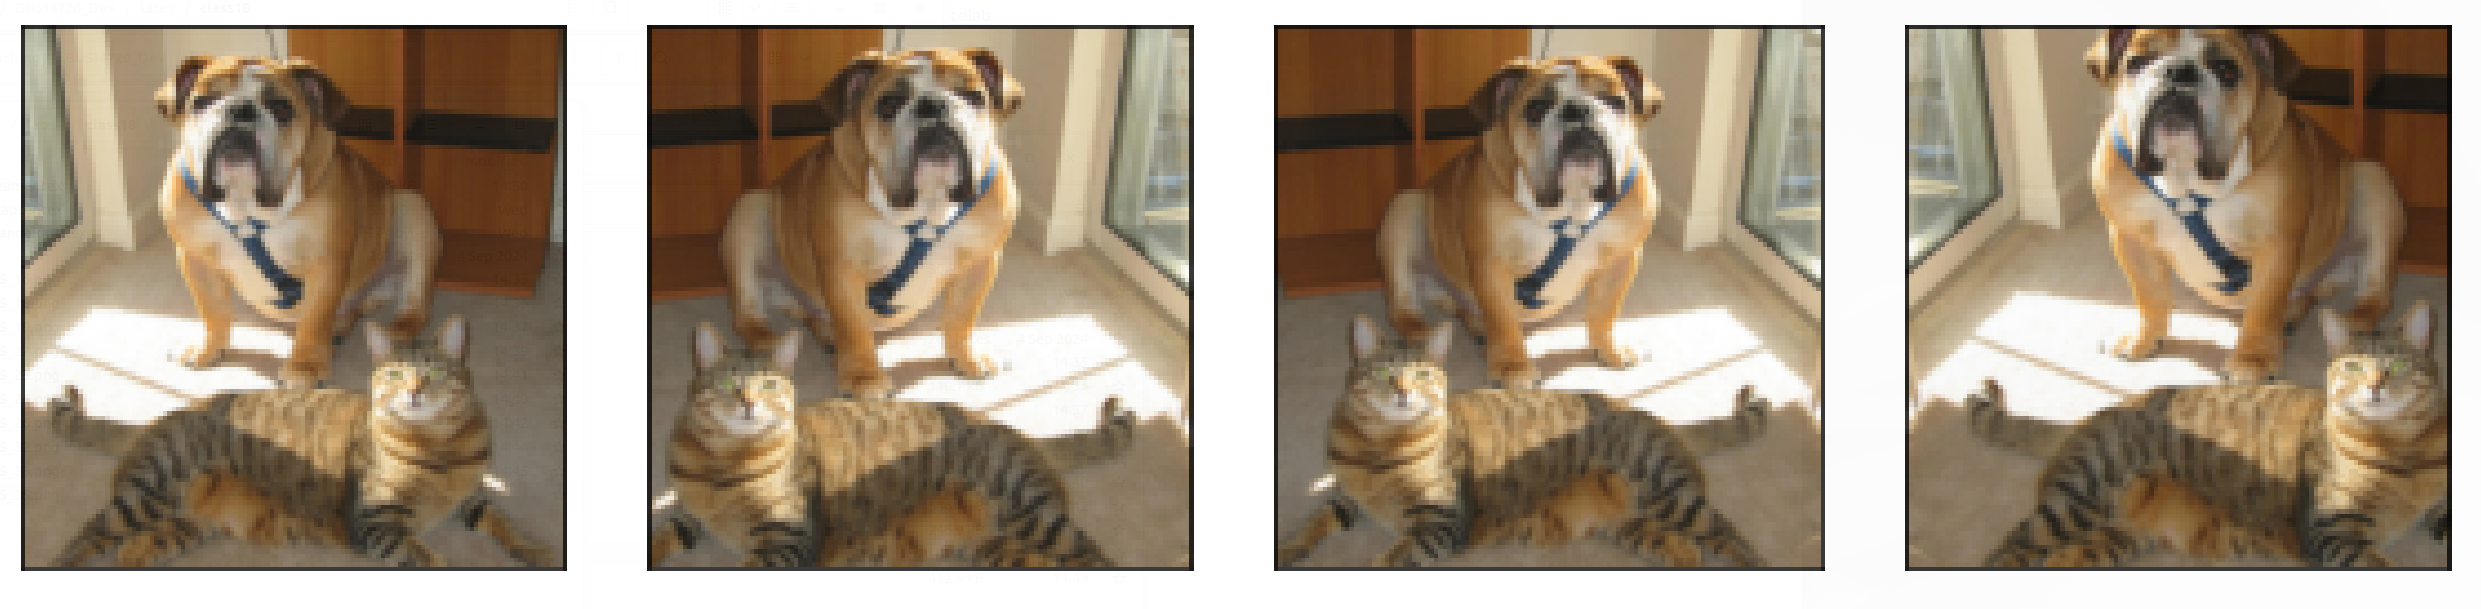
\includegraphics[width=\textwidth]{murphy_19_01.png} \\

\scriptsize Source: Murphy Fig. 19.1
\normalsize

\begin{block}{Examples in Vision}
\begin{itemize}
   \item Geometric transformations
   \begin{itemize}
      \item Rotate, Flip, Crop, Translate
   \end{itemize}
   \item Color space transformations
   \begin{itemize}
      \item Brightness, contrast, saturation
   \end{itemize}
   \item Noise injection
   \begin{itemize}
      \item Gaussian noise, random pixels, black pixels
   \end{itemize}
   \item Kernal filters
   \begin{itemize}
      \item Blurring or smoothing
   \end{itemize}
\end{itemize}
\end{block}
\end{frame}

\begin{frame}{Data Augmentation \small [cont'd]}

\begin{block}{Examples in Text}
\begin{itemize}
   \item Character, word or sentence shuffling
   \item Word replacement with synonyms or similar words
   \item Random word insertion and deletion
   \item Noise insertion at embedding level
   \item Forward-backward translation
\end{itemize}
\end{block}
\end{frame}

\begin{frame}{Data Augmentation \small [cont'd]}
\begin{block}{Examples in Tabular Data}
\begin{itemize}
   \item SMOTE, SMOTE-NC (''Synthetic Minority Oversampling Technique'')
   \item AdaSyn (''Adaptive synthetic sampling'')
   \item Variational autoencoders
\end{itemize}
\end{block}

\begin{columns}
\begin{column}{0.2\textwidth}
\textbf{SMOTE principles}
\end{column}
\begin{column}{0.8\textwidth}
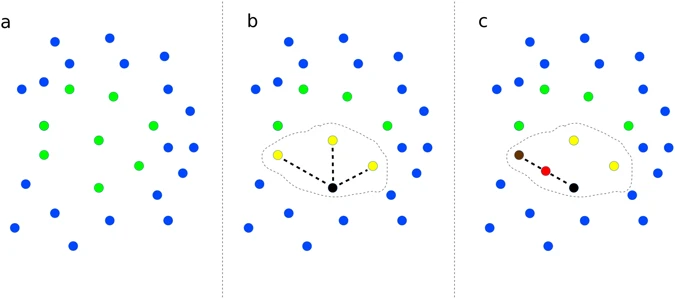
\includegraphics[width=\textwidth]{smote.png} 
\end{column}
\end{columns}

\centering

\tiny Source: Schubach, M., Re, M., Robinson, P.N. et al. Imbalance-Aware Machine Learning for Predicting Rare and Common Disease-Associated Non-Coding Variants. Sci Rep 7, 2959 (2017). https://doi.org/10.1038/s41598-017-03011-5 (CC-BY-4.0)
\normalsize
\end{frame}

\begin{frame}{Transfer Learning}

\begin{block}{Ideas}
\begin{itemize}
   \item Transfer learned models to related domains
   \begin{itemize}
      \item Example: Use CNN for classifying cars to classify trucks
   \end{itemize}
   \item For data-poor tasks similar to other tasks
   \begin{itemize}
      \item Example: Classify endangered bird species with CNN trained on common birds
   \end{itemize}
   \item To reduce training effort/cost
   \begin{itemize}
      \item Example: Adapt pre-trained CNN to recognize organization-specific images
   \end{itemize}
   \item Related to multi-objective learning/optimization
\end{itemize}
\end{block}

\begin{block}{Phases}
\begin{enumerate}
   \item \emph{Pretraining} on large \emph{source data set}
   \item \emph{Fine-tuning} on smaller \emph{target data set}
\end{enumerate}
\end{block}
\end{frame}

\begin{frame}{Transfer Learning \small [cont'd]}

\begin{center}
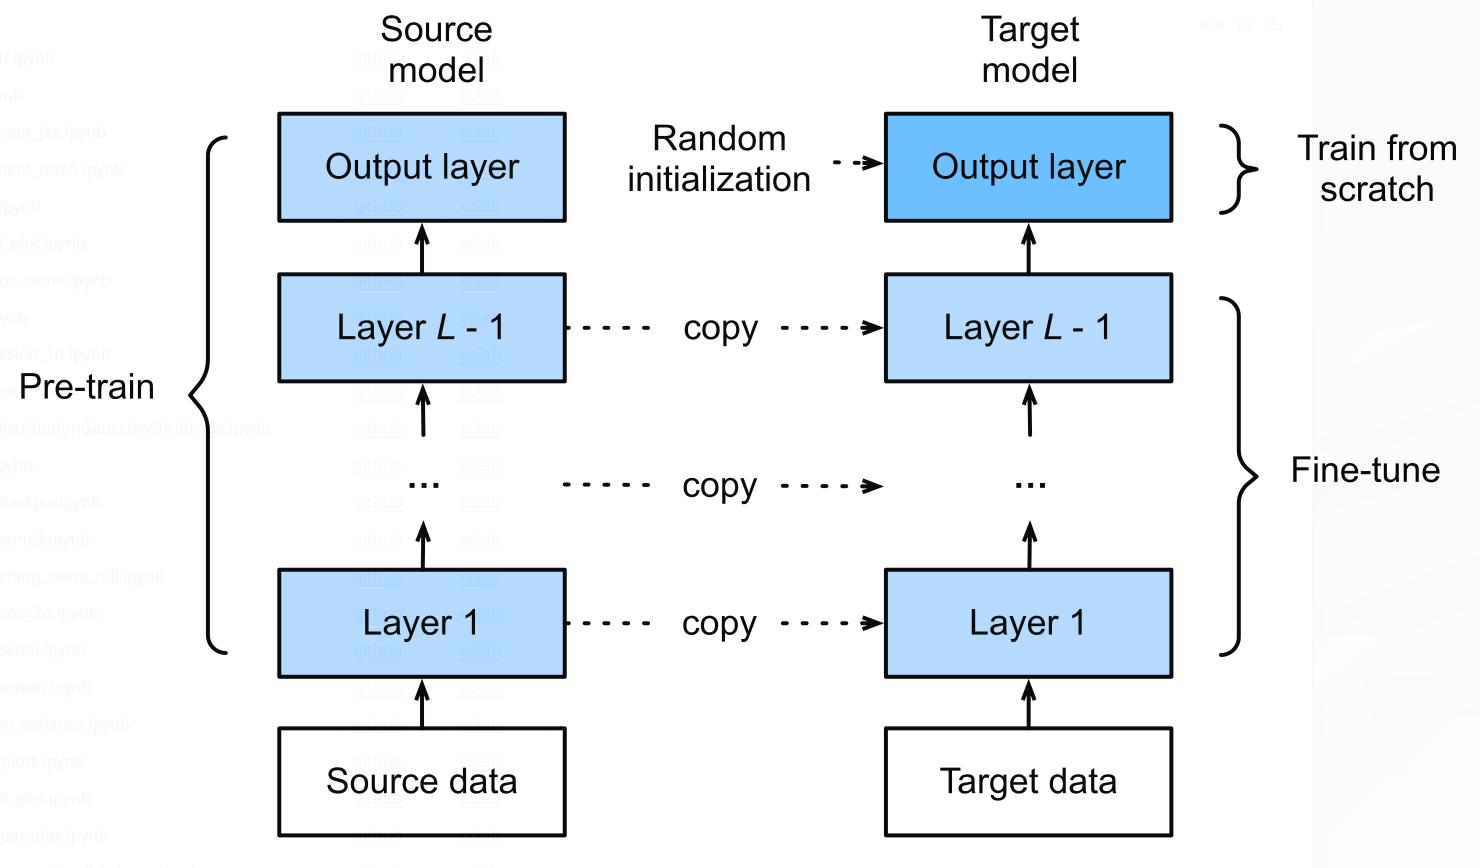
\includegraphics[width=0.8\textwidth]{murphy_19_02.png} \\
\scriptsize Source: Murphy Fig 19.2 (CC-BY-NC-ND) from \url{https://github.com/d2l-ai/d2l-en} (CC-BY 4.0) \normalsize
\end{center}

\begin{block}{Options}
\begin{itemize}
   \item Do not fine-tune pre-trained layers (fix/freeze)
   \item Fine-tune pre-trained layers using small learning rate
\end{itemize}
\end{block}   
\end{frame}

\begin{frame}[fragile]{Data Augmentation in Python}

Load Tensorflow example data set:
\begin{pythoncode}
import keras
from keras import layers
import tensorflow_datasets as tfds

# Load a Tensorflow example image data set
train_ds, test_ds = tfds.load(
    "cats_vs_dogs",
    split=["train[:75%]", "train[75%:100%]"],
    as_supervised=True)
\end{pythoncode}

Resize images to same size using Keras Resizing layer:
\begin{pythoncode}
# Create Resizing layer
resize_fn = keras.layers.Resizing(150, 150)

# Apply resizing layer to data sets
train_ds = train_ds.map(lambda x, y: (resize_fn(x), y))
test_ds = test_ds.map(lambda x, y: (resize_fn(x), y))
\end{pythoncode}
\end{frame}

\begin{frame}[fragile]{Data Augmentation in Python \small [cont'd]}
Data augmentation using Keras layers:
\begin{pythoncode}
# Define a sequential model of random transformation layers
augmentation = keras.models.Sequential([
    layers.RandomFlip("horizontal"),
    layers.RandomTranslation(.2, .2, fill_mode="reflect"),
    layers.RandomRotation(0.2, fill_mode="reflect"),
    layers.RandomZoom(.2, .2, fill_mode="reflect"),
    layers.RandomContrast(0.2),
    layers.RandomBrightness(0.2)])

# Apply augmentation model to training data
train_ds = train_ds.map(lambda x, y: (augmentation(x), y))
\end{pythoncode}

\begin{block}{}
\small
\begin{itemize}
   \item This example applies all layers to all training images; consider applying single transformations to an image or random combinations of transformations
   \item This example replaces the data set with the transformed images; consider adding the transformed images to the data set
\end{itemize}
\end{block}
\end{frame}

\begin{frame}[fragile]{Transfer Learning in Python}
Load an image classification model and its  pre-trained  weights from Keras applications \emph{without} the top classification layer:
\begin{pythoncode}
base_model = keras.applications.Xception(
    weights="imagenet",
    input_shape=(150, 150, 3),
    include_top=False)
\end{pythoncode}

Freeze/fix the model's parameters, that is, make not trainable:
\begin{pythoncode}
base_model.trainable = False
\end{pythoncode}
\end{frame}

\begin{frame}[fragile]{Transfer Learning in Python \small [cont'd]}

Create a new layer with specific input image shape:
\begin{pythoncode}
# Create new input model
inputs = keras.Input(shape=(150, 150, 3))
# Pre-trained Xception weights requires input scaling
# from [0, 255] to [-1., +1.]
scale_layer = keras.layers.Rescaling(scale=1/127.5, offset=-1)
x = scale_layer(inputs)
\end{pythoncode}

Add a new bottom layer for classification to the model. Make sure the base model is not trained:
\begin{pythoncode}
x = base_model(x, training=False)
x = keras.layers.GlobalAveragePooling2D()(x)
x = keras.layers.Dropout(0.2)(x)
outputs = keras.layers.Dense(1)(x)

# Complete model has inputs and outputs
model = keras.Model(inputs, outputs)
# Not all parameters are trainable
model.summary(show_trainable=True)
\end{pythoncode}
\end{frame}

\begin{frame}[fragile]{Transfer Learning in Python \small [cont'd]}

Compile and fit the new model (training only the classification layers) with default learning rate for optimizer:
\begin{pythoncode}
model.compile(
    optimizer=keras.optimizers.Adam(),
    loss=keras.losses.BinaryCrossentropy(from_logits=True),
    metrics=[keras.metrics.BinaryAccuracy()],
)
model.fit(train_ds.batch(64), epochs=2, 
          validation_data=test_ds.batch(64))
\end{pythoncode}
\begin{block}{}
Only a few epochs are needed
\end{block}

\end{frame}

\begin{frame}[fragile]{Transfer Learning in Python \small [cont'd]}

Fine-tune the base model with a very small learning rate:
\begin{pythoncode}
# Make all parameters trainable
base_model.trainable = True
# Now all parameters are trainable
model.summary(show_trainable=True)

# Very small learning rate
model.compile(
    optimizer=keras.optimizers.Adam(1e-5),
    loss=keras.losses.BinaryCrossentropy(from_logits=True),
    metrics=[keras.metrics.BinaryAccuracy()],
)
model.fit(train_ds.batch(64), epochs=2, 
          validation_data=test_ds.batch(64))
\end{pythoncode}

\begin{block}{}
Only a few epochs are needed
\end{block}
\end{frame}

\begin{frame}{Data Augmentation and Transfer Learning in Python}

Adapted from: 

\small\url{https://keras.io/guides/transfer_learning/}\normalsize \\

Implementation available on the following GitHub repo:

\small\url{https://github.com/jevermann/busi4720-ai}\normalsize \\

The project can be cloned from this URL:

\small\url{https://github.com/jevermann/busi4720-ai.git}\normalsize
\end{frame}

\begin{frame}{Adapters}

\begin{block}{Fine-tuning problems:}
\begin{itemize}
\item Fine-tuning may be slow for large model sizes
\item Parameters may diverge too far from prior values
\item New tasks require new fine-tuning of all parameters
\end{itemize}
\end{block}

\begin{block}{Adapters:}
\begin{itemize}
\item Fix/freeze pre-trained parameters
\item Add additional model layers with their own parameters (''adapters'')
\end{itemize}
\end{block}
\end{frame}

\begin{frame}{Adapters \small [cont'd]}
\begin{block}{Examples}
  \begin{enumerate}[(a)]
     \item Adapter in transformer layer
     \item Adapter in ResNet
  \end{enumerate}
\end{block}

\centering
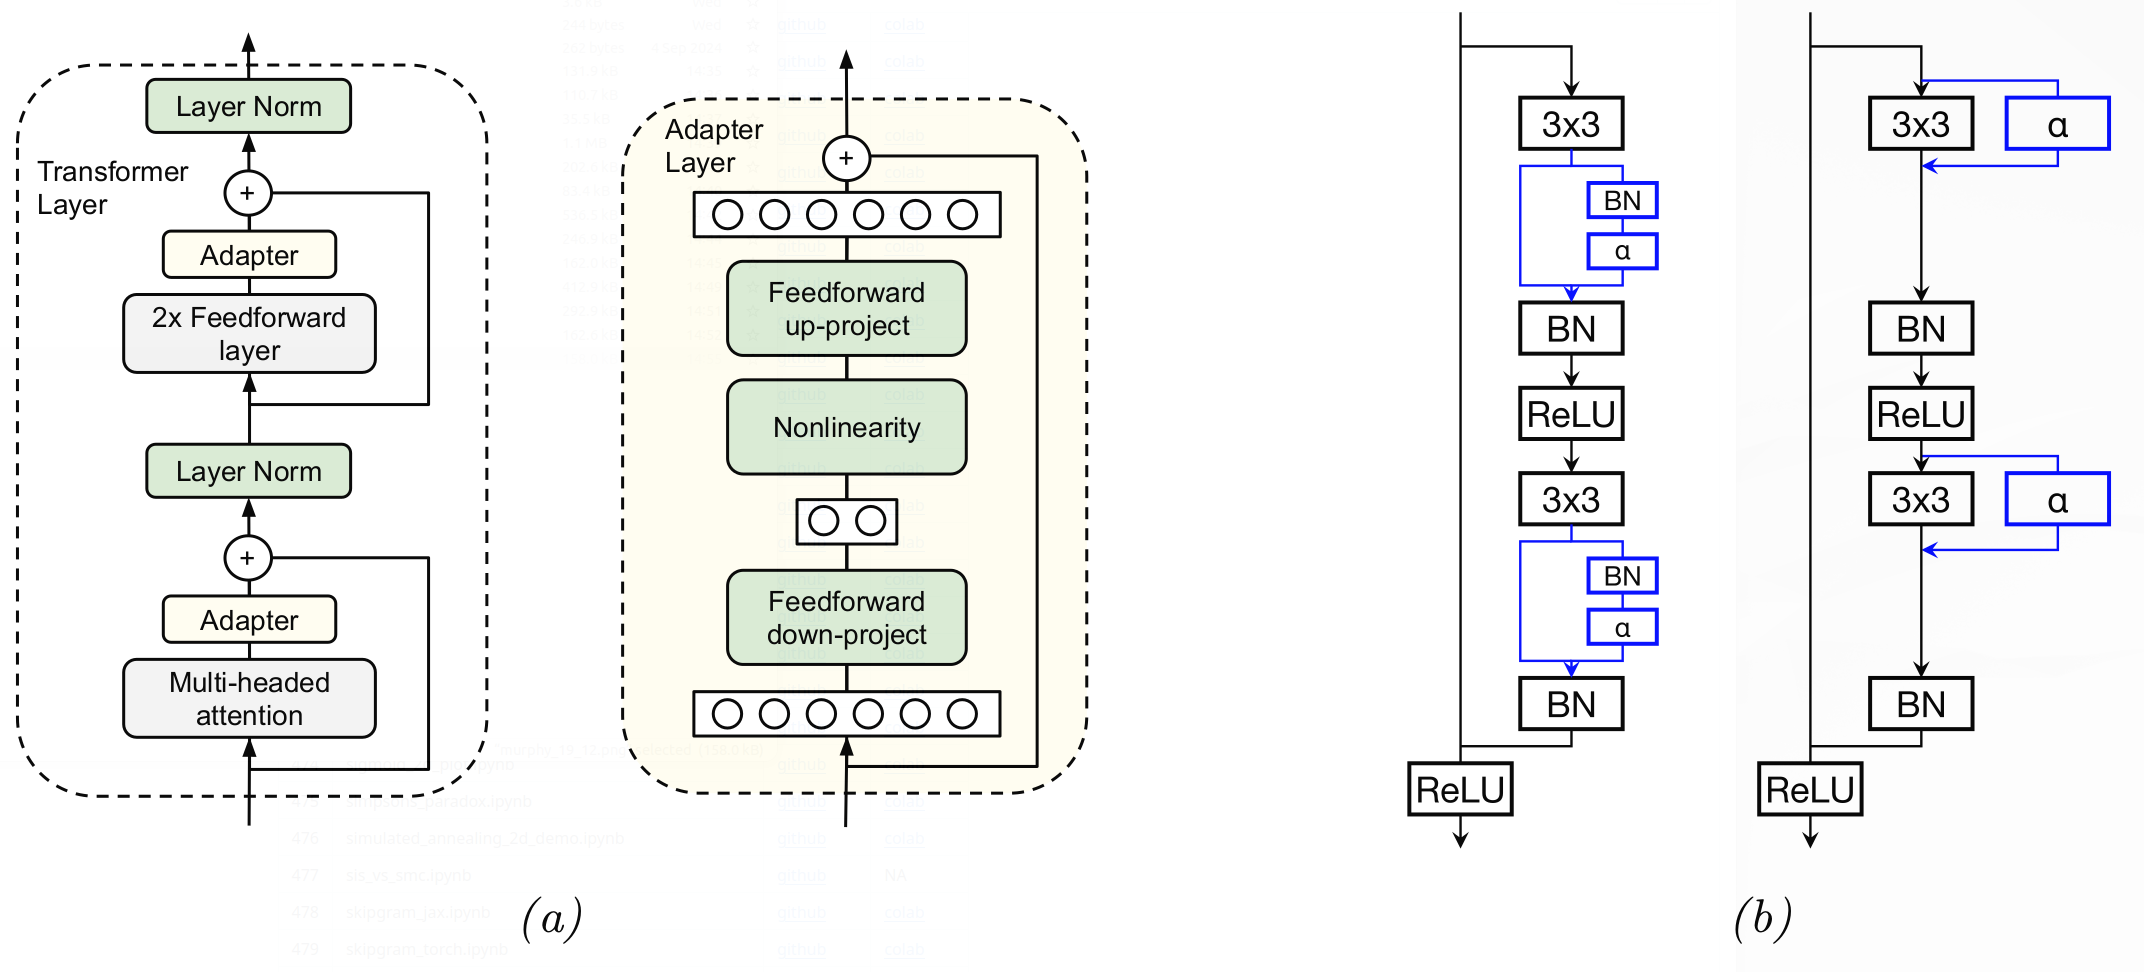
\includegraphics[width=\textwidth]{murphy_19_03.png} \\
\scriptsize Source: Murphy Fig. 19.3 \normalsize
\end{frame}

\begin{frame}{Attention}
\begin{itemize}
  \item A set of $m$ key vectors $K$ and value vectors $V$
  \item A query vector $Q$
  \item Attention score function $a$ determines similarity of keys to query
  \item Determine weights for values based on attention scores
\end{itemize}

\centering
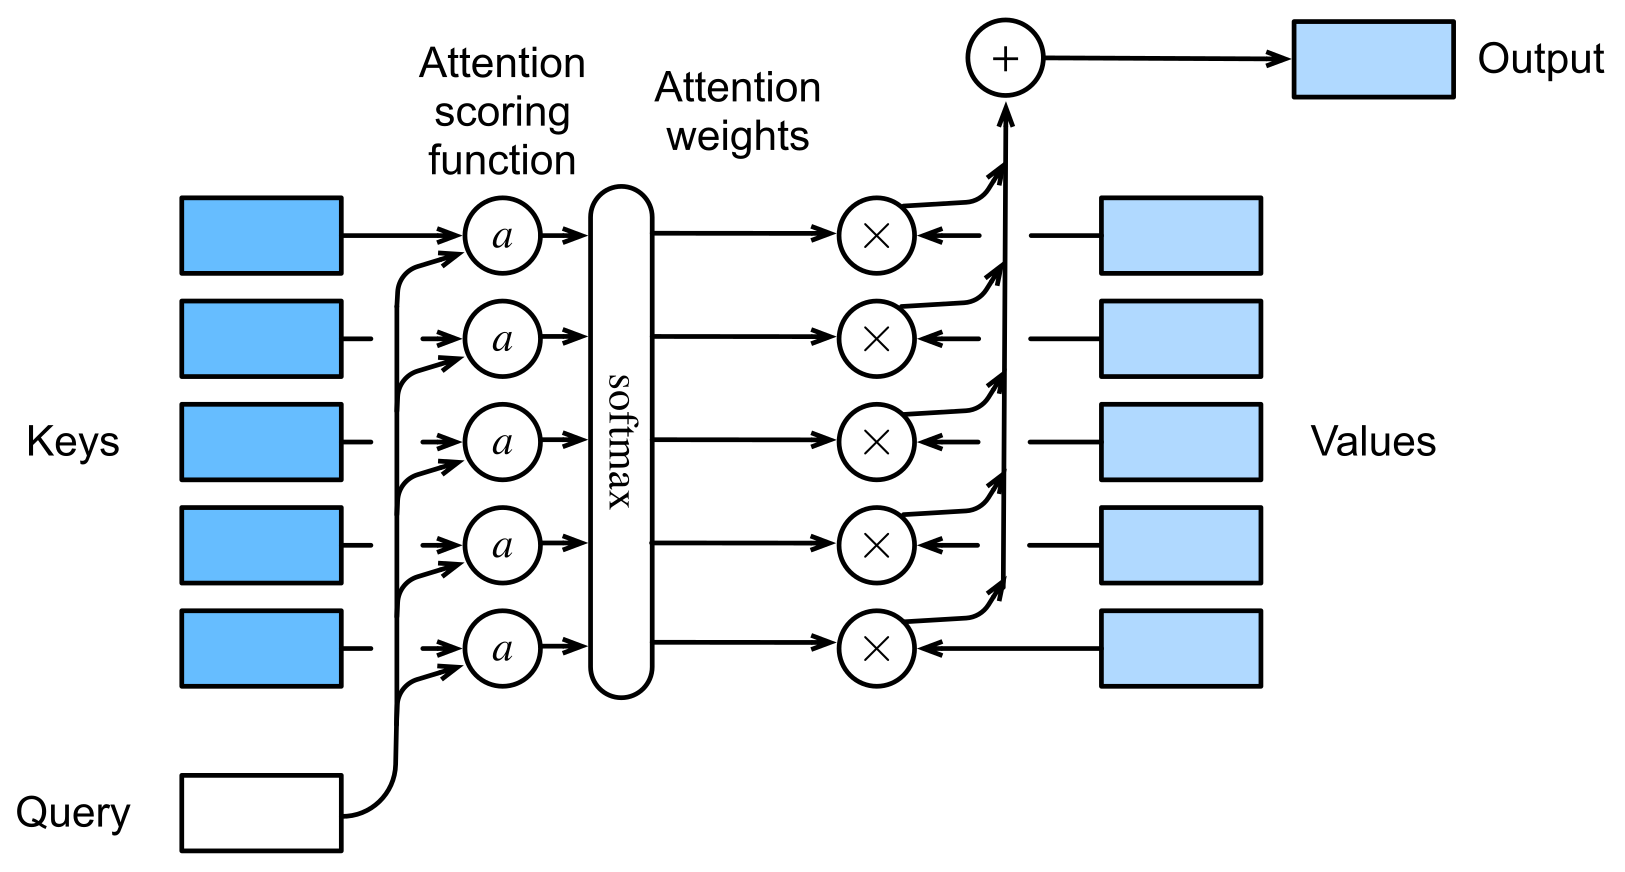
\includegraphics[height=1.75in]{murphy_15_16.png} \\

\scriptsize Source: Murphy, Fig. 15.16 \normalsize
\end{frame}

\begin{frame}{Attention \small [cont'd]}
\begin{block}{Scaled Dot-Product Attention}
\begin{align*}
\operatorname{Attn}(Q, K, V) = \operatorname{softmax}\left(\frac{Q K^T}{\sqrt{d_k}} \right) V
\end{align*}
\end{block}

%\begin{block}{Masked Attention}
%\begin{align*}
%\operatorname{Attn}(Q, K, V) = \operatorname{softmax}\left(\frac{Q K^T}{\sqrt{d_k}} + M \right) V
%\end{align*}
%$M$ is an upper triangular marix with 0 on and below the diagonal.
%\end{block}
\end{frame}

\begin{frame}{Attention in Seq2Seq Models}

\begin{itemize}
  \item Encoder -- Decoder network
  \item Allow decoder access to input sequence, but word (token) order need not be preserved, must infer \emph{alignment}
\end{itemize}
\centering

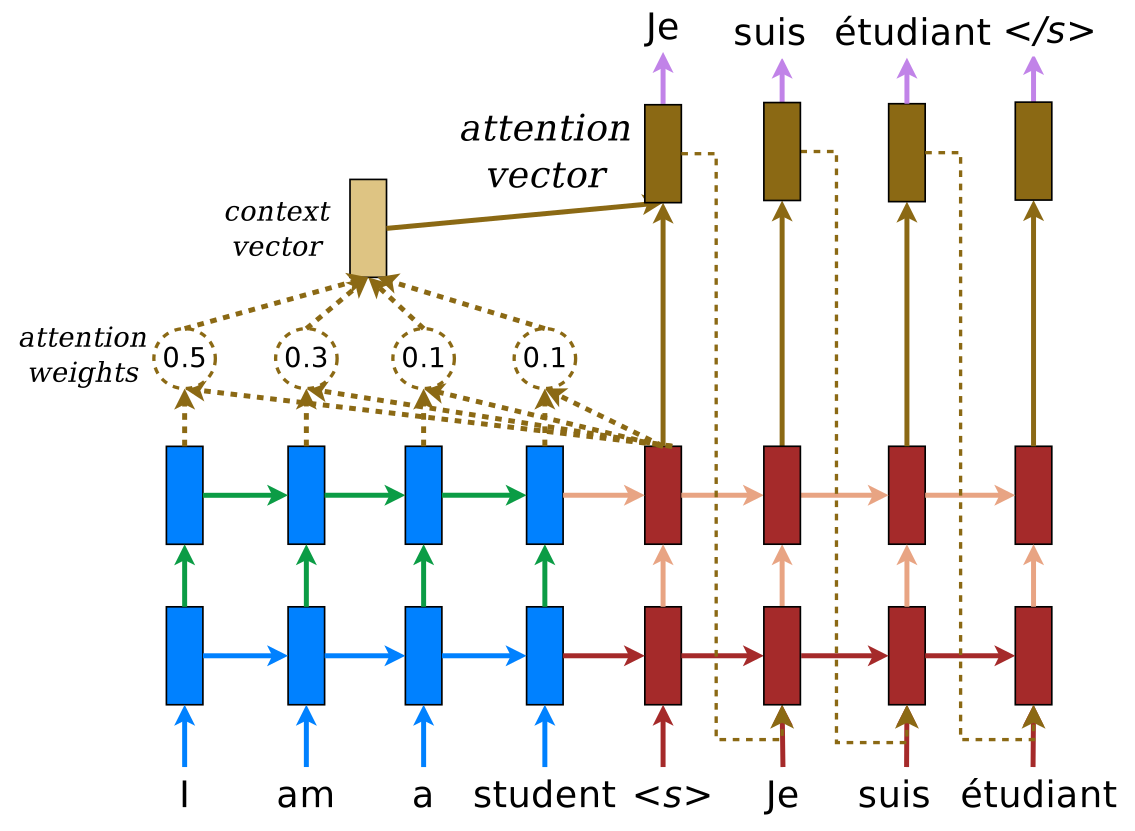
\includegraphics[height=2in]{murphy_15_18.png} \\

\scriptsize Source: Murphy, Fig. 15.18 \normalsize
\end{frame}

\begin{frame}{Attention in Seq2Seq Models}
Instead of fixed context vector for decoder:
\begin{align*}
c &= h_T^e
\intertext{now:}
c_t &= \operatorname{Attn}(Q = h_{t-1}^d, K = h^e, V = h^e)
\end{align*}

Query $Q$ is the hidden state of decoder, keys $K$ and values $V$ are hidden states from encoder
\end{frame}

\begin{frame}{Attention in Seq2Seq Models}
\textbf{Example:} Attention in English -- Spanish translation

\begin{center}
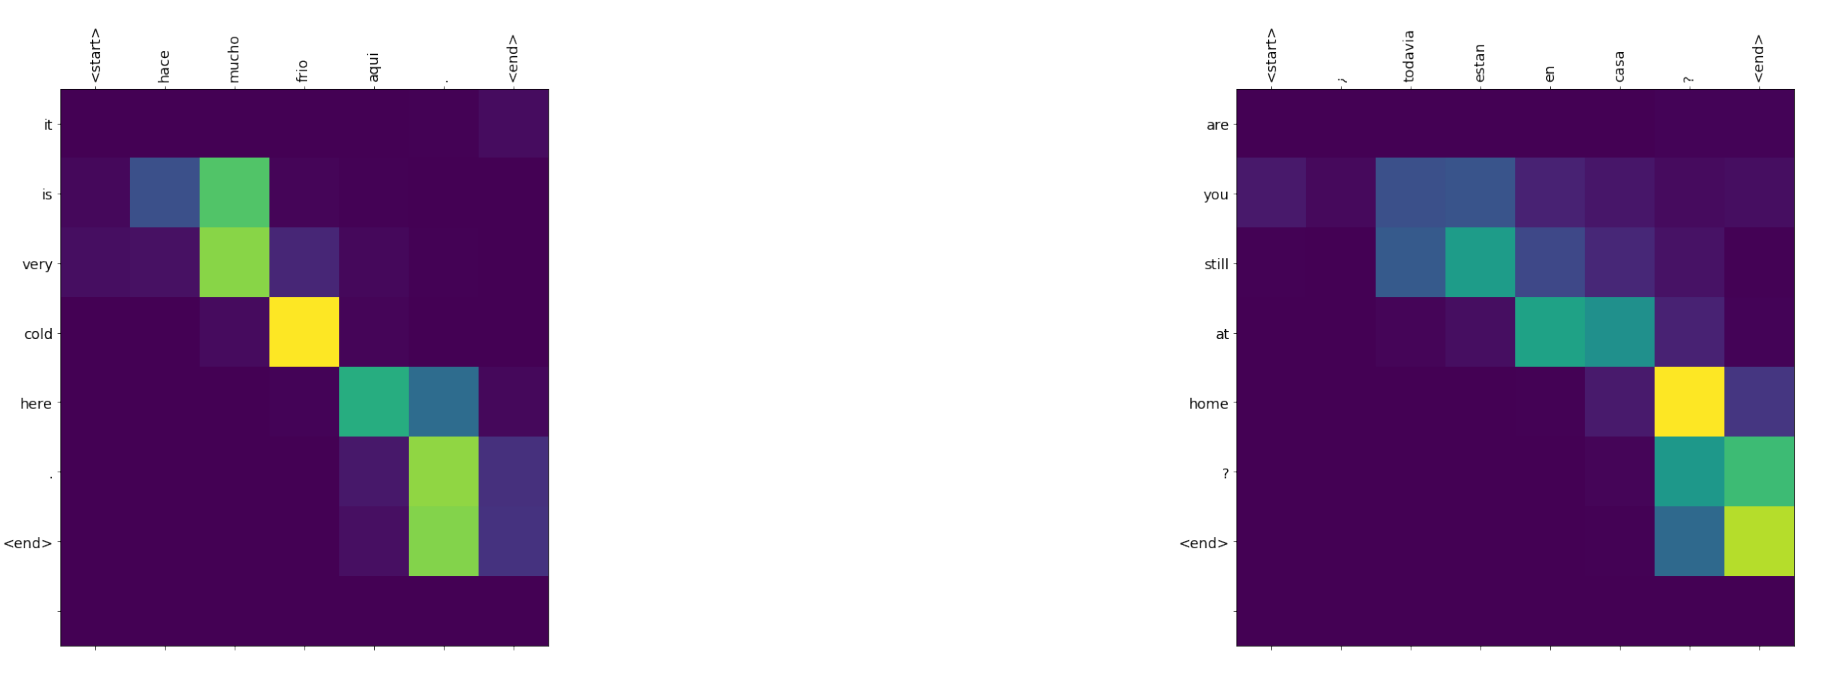
\includegraphics[width=\textwidth]{murphy_15_19.png} \\

\scriptsize Source: Murphy, Fig. 15.19 \normalsize
\end{center}
\end{frame}

\begin{frame}{Multi-Headed Attention}
\begin{align*}
\operatorname{MultiHead}(Q, K, V) &= W_o \operatorname{Concat} (h_1, \ldots h_h) = W_o \begin{pmatrix} h_1 \\ \vdots \\ h_n \end{pmatrix} 
\intertext{where each head $h_i$ is defined as:}
h_i &= \operatorname{Attn}(QW_i^{(Q)}, KW_i^{(K)}, VW_i^{(V)})
\end{align*}
and $W_i^{(Q)}, W_i^{(K)}, W_i^{(V)},$ and $W^{(O)}$ are trainable weight matrices.

\begin{center}
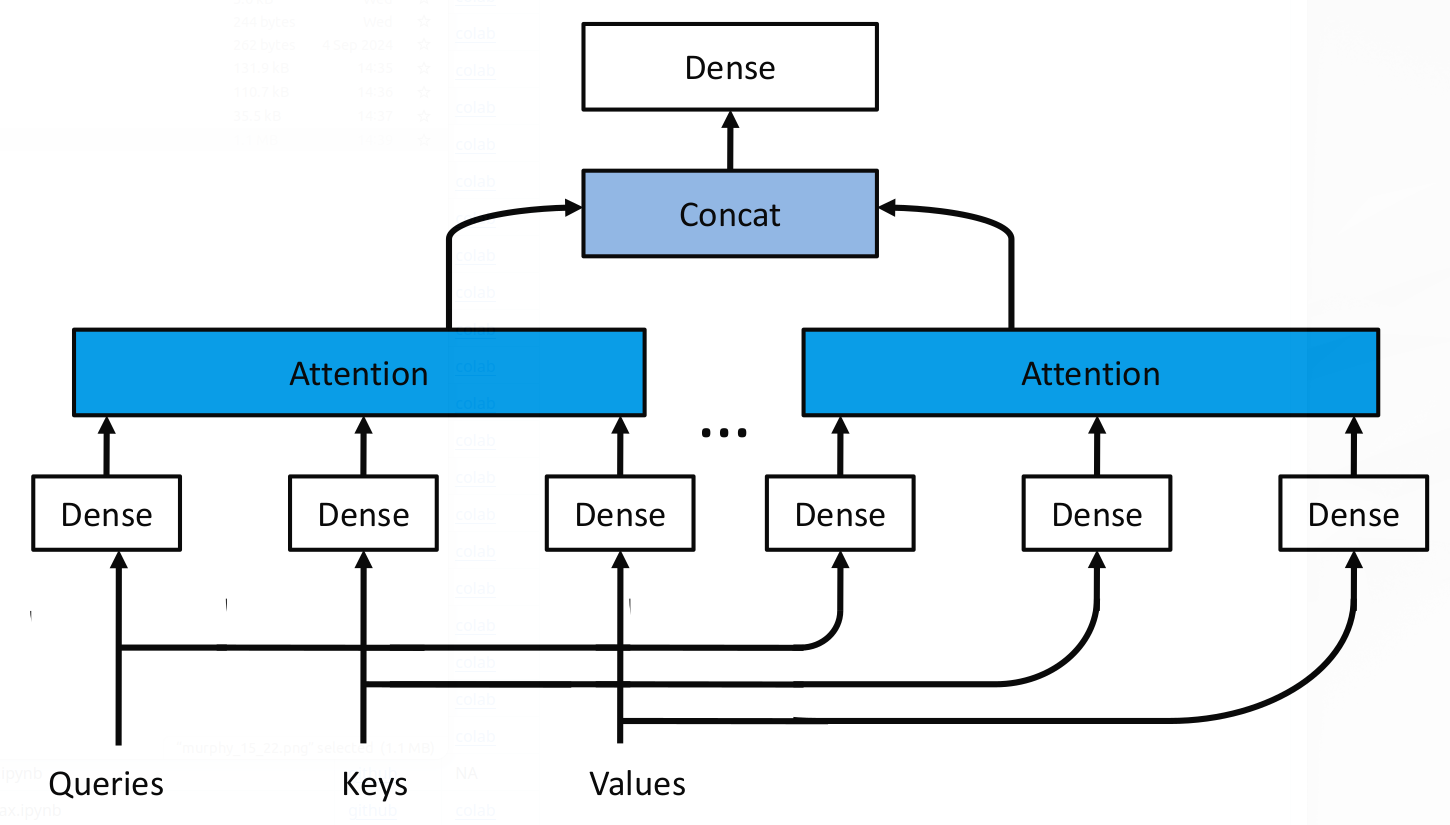
\includegraphics[height=1.25in]{murphy_15_24.png} \\

\scriptsize Source: Murphy, Fig. 15.24 \normalsize
\end{center}
\end{frame}

\begin{frame}{Self-Attention}
Query, keys, and values come from the same model, i.e. from the encoder or decoder.
\begin{align*}
y_i = \operatorname{Attn}(x_i, X, X)
\end{align*}
Where $y_1$ is output $i$, $x_i$ is input $i$, and the matrix $X$ is the matrix of all $n$ inputs in the sequence. 

\begin{center}
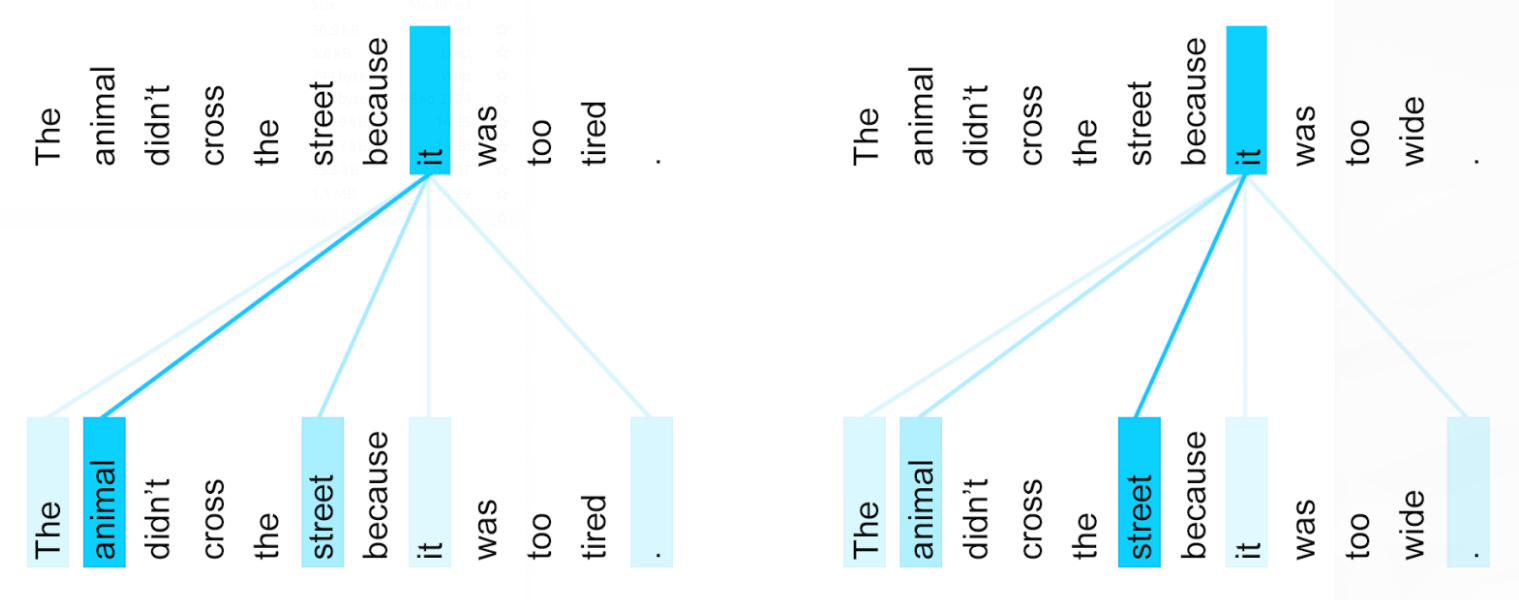
\includegraphics[height=1.5in]{murphy_15_23.png} \\

\scriptsize Source: Murphy, Fig. 15.23 \normalsize
\end{center}
\end{frame}

\begin{frame}{Positional Encoding}
Model must know the order words (tokens) occur in. Positional encodings provide this. 
\begin{align*}
&p_{i, 2j} = \sin \left( \frac{i}{C^{2j/d}} \right), \ p_{i, 2j+1} = \cos \left( \frac{i}{C^{2j/d}} \right) \ \forall j \in [1 \ldots d/2]
\end{align*}
\begin{itemize}
\item $d$ is the chosen dimensionality of the positional encoding.
\item $C$ is the maximum vocabulary size.
\end{itemize}

For example, if $d=4$ the i-th row is:
\begin{align*}
&p_i = [ \sin(\frac{i}{C^{0/4}}), \cos(\frac{i}{C^{0/4}}), \sin(\frac{i}{C^{2/4}}), \cos(\frac{i}{C^{2/4}}) ]
\end{align*}

Combine with word embeddings $X$:
\begin{align*}
&\operatorname{POS}(\operatorname{Embed}(X)) = X + P
\end{align*}
\end{frame}

\begin{frame}{Positional Encoding \small [cont'd]}
\begin{itemize}
\item Example for 1000 positions (rows) and embedding dimension of 64. 
\item Each row is a real-valued vector representing its location in the sequence:
\end{itemize}
\begin{center}
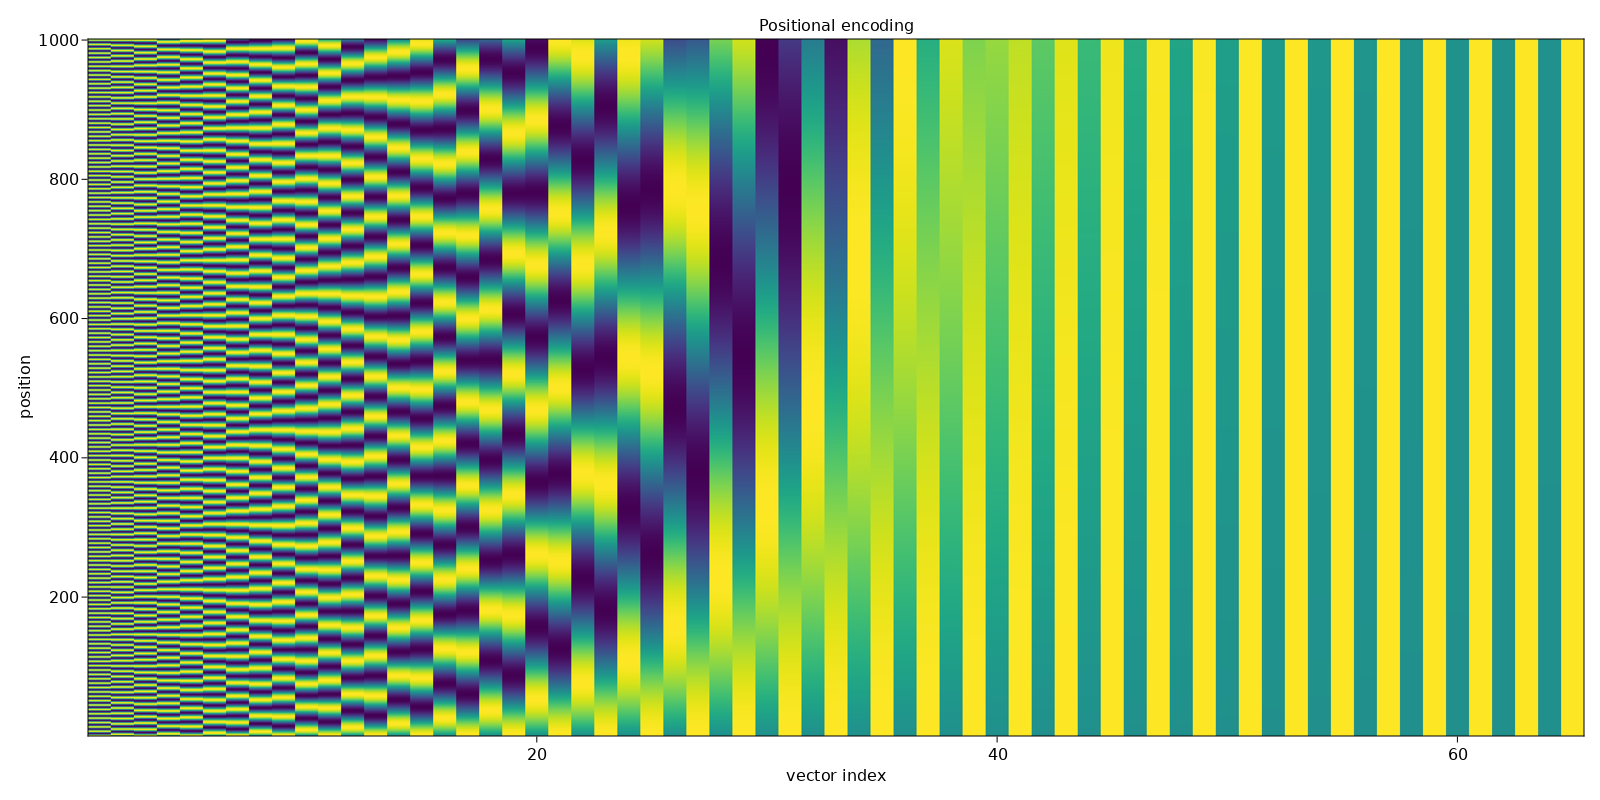
\includegraphics[height=1.75in]{Positional_encoding.png} \\

\tiny Source: \url{https://commons.wikimedia.org/wiki/File:Positional_encoding.png} \normalsize
\end{center}
\end{frame}

\begin{frame}[fragile]{Positional Encoding in Python}
Define weights:
\begin{pythoncode}
import numpy as np

def position_encoding_matrix(seq_len, d, C=10000):
    P = np.zeros((seq_len, d))
    for i in range(seq_len):
        for j in np.arange(int(d / 2)):
            denominator = np.power(C, 2 * i / d)
            P[i, 2 * j] = np.sin(i / denominator)
            P[i, 2 * j + 1] = np.cos(i / denominator)
    return P
\end{pythoncode}
\end{frame}

\begin{frame}[fragile]{Positional Encoding in Python \small [cont'd]}
Define Keras layer:
\begin{pythoncode}
class TokenAndPositionEmbedding(layers.Layer):
    def __init__(self, maxlen, vocab_size, embed_dim):
        super().__init__()
        # Generate the positional encoding weights
        position_embedding_matrix = \
            position_encoding_matrix(maxlen, embed_dim)
        # Trainable token embedding layer
        self.token_emb = layers.Embedding(
            input_dim=vocab_size, output_dim=embed_dim)
        # Positional embedding with positional 
        # encoding weights is not trainable
        self.pos_emb = layers.Embedding(
            input_dim=maxlen, output_dim=embed_dim,
            weights=[position_embedding_matrix],
            trainable=False
        )

    def call(self, x):
        maxlen = tf.shape(x)[-1]
        positions = tf.range(0, maxlen, 1)
        # Return token plus position embedding
        return self.token_emb(x) + self.pos_emb(positions)
\end{pythoncode}
\end{frame}


\begin{frame}[fragile]{Transformer}

Encoder uses multi-headed self-attention:

\begin{columns}
\begin{column}{.75\textwidth}
\begin{textcode}
def EncoderBlock(X):
  Z = LayerNorm(MultiHeadAttn(Q=X,K=X,V=X)+X)
  E = LayerNorm(FeedForward(Z) + Z)
  return E
\end{textcode}

\begin{textcode}
def Encoder(X, N):
  E = POS(Embed(X))
  for n in range(N):
    E = EncoderBlock(E)
  return E
\end{textcode}
\end{column}
\begin{column}{.3\textwidth}
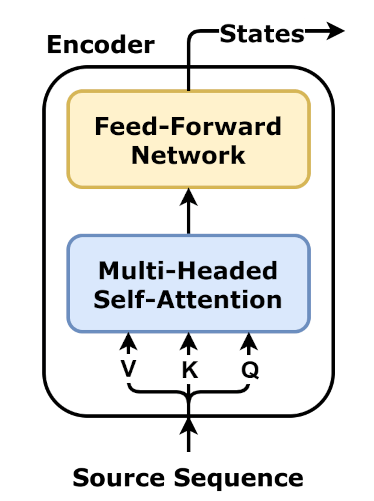
\includegraphics[width=\textwidth]{Transformer,_one_encoder_block.png} \\

\tiny \url{https://commons.wikimedia.org/wiki/File:Transformer,_one_encoder_block.png}
\end{column}
\end{columns}
\end{frame}

\begin{frame}[fragile]{Transformer}

Decoder uses multi-headed self-attention:

\begin{columns}
\begin{column}{.75\textwidth}
\begin{textcode}
def DecoderBlock(Y, E):
  Z = LayerNorm(MultiHeadAttn(Q=Y,K=Y,V=Y)+Y)
  Z' = LayerNorm(MultiHeadAttn(Q=Z,K=E,V=E)+Z)
  D = LayerNorm(FeedForward(Z') + Z')
  return D
\end{textcode}

\begin{textcode}
def Decoder(Y, E, N):
  D = POS(Embed(Y))
  for n in range(N):
    D = DecoderBlock(D,E)
  return D
\end{textcode}
\end{column}
\begin{column}{.3\textwidth}
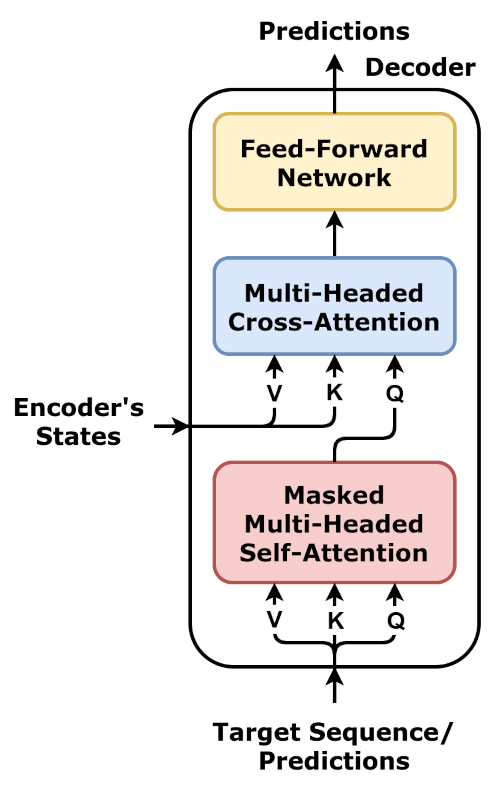
\includegraphics[width=\textwidth]{Transformer,_one_decoder_block.png} \\

\tiny \url{https://commons.wikimedia.org/wiki/File:Transformer,_one_decoder_block.png}
\end{column}
\end{columns}
\end{frame}

\begin{frame}{Transformer \small [cont'd]}
\centering

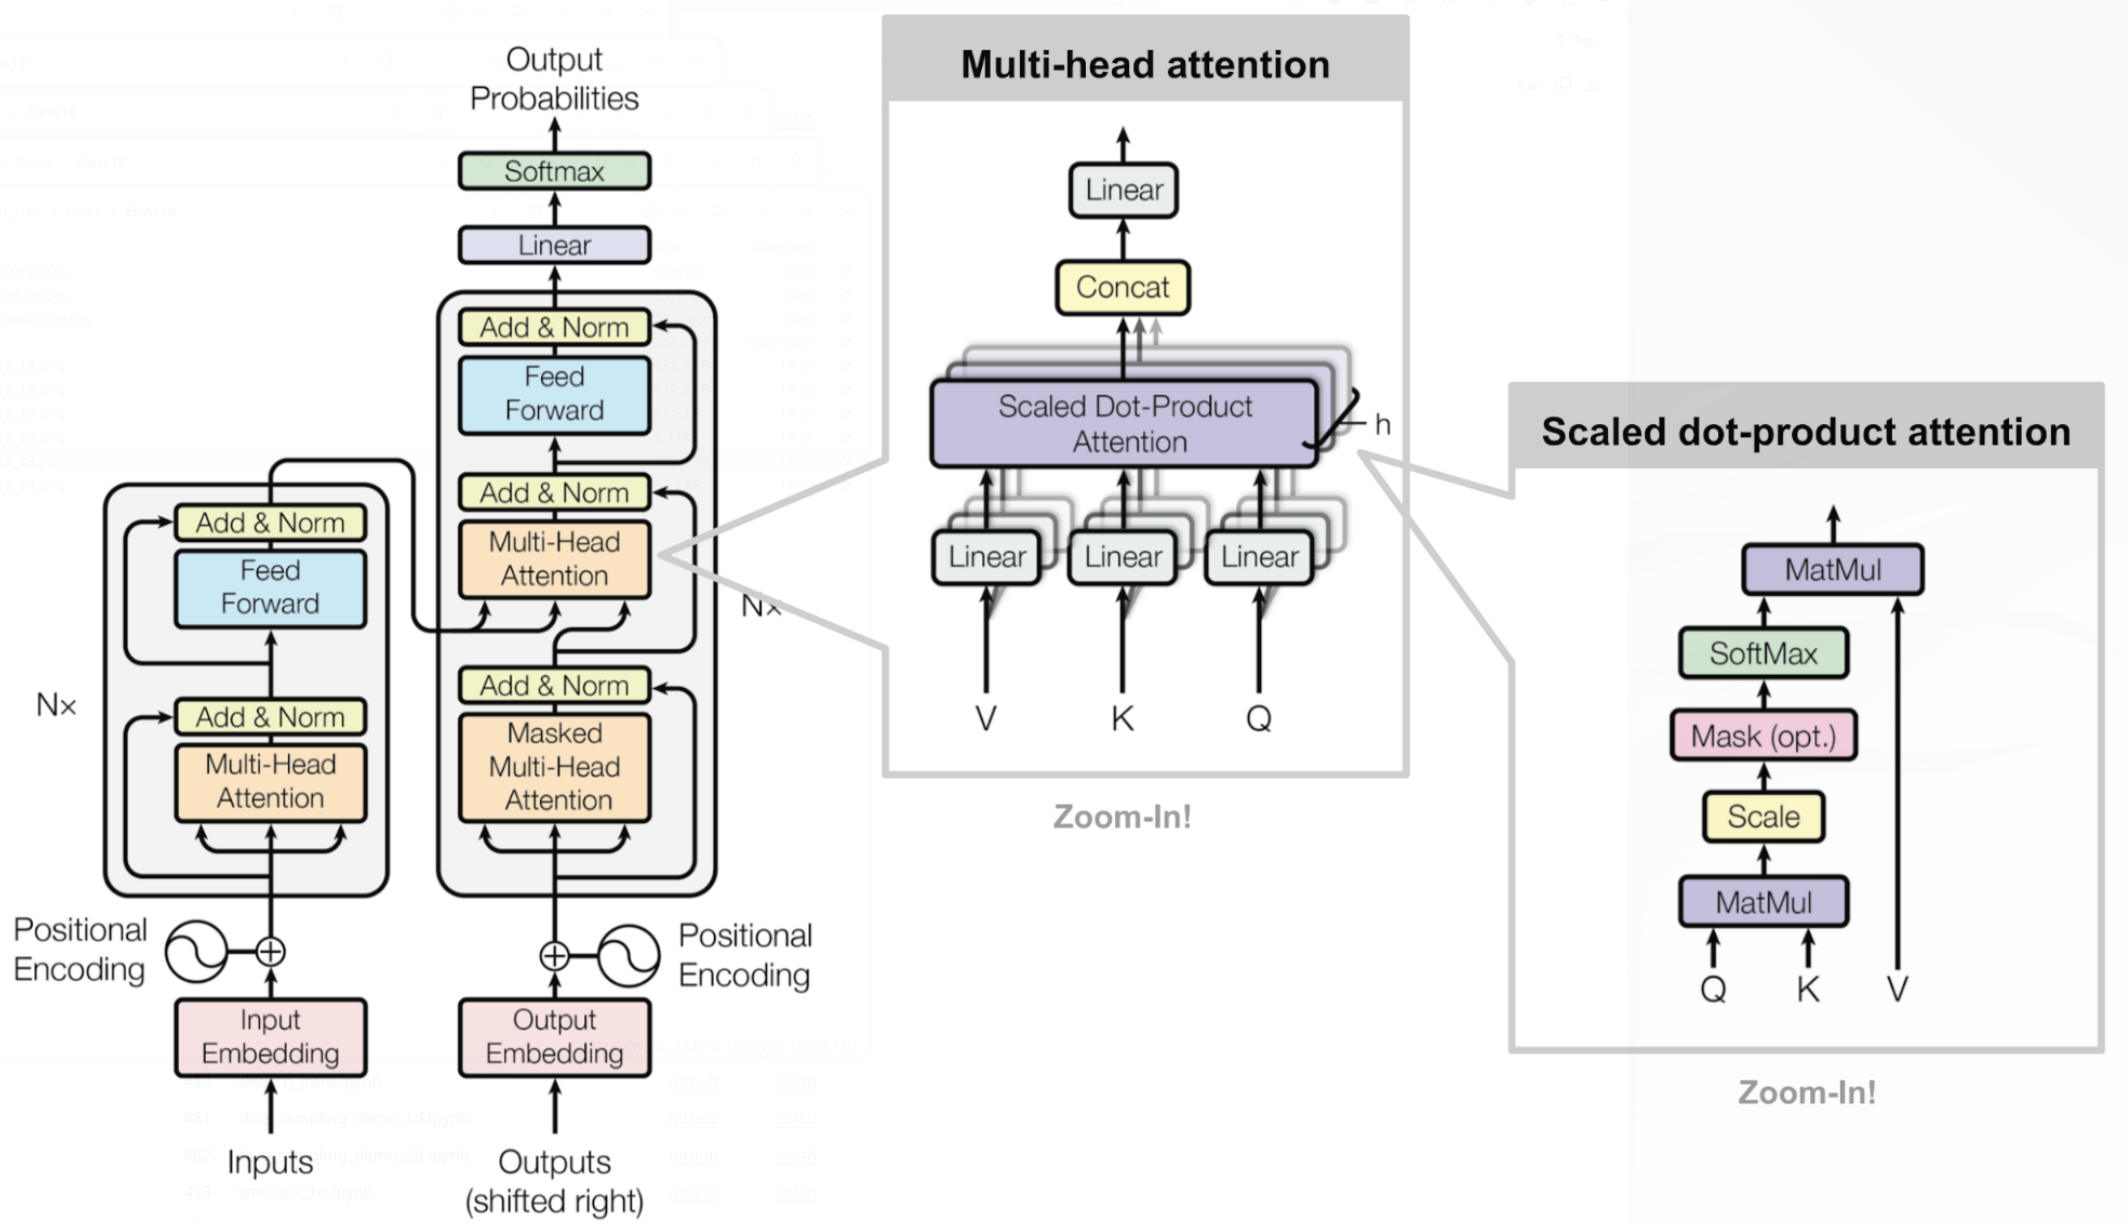
\includegraphics[width=\textwidth]{murphy_15_26.png} \\

\scriptsize Source: Murphy, Fig. 15.26 \normalsize
\end{frame}

\begin{frame}[fragile]{Transformer Encoder in Python}

\begin{pythoncode}
class TransformerBlock(layers.Layer):
    def __init__(self, embed_dim, num_heads, ff_dim, rate=0.1):
        super().__init__()
        self.att = layers.MultiHeadAttention(num_heads, 
                                             embed_dim)
        self.ffn = keras.Sequential([
                layers.Dense(ff_dim, activation="relu"),
                layers.Dense(embed_dim)])
        self.norm1 = layers.LayerNormalization()
        self.norm2 = layers.LayerNormalization()
        self.dropout1 = layers.Dropout(rate)
        self.dropout2 = layers.Dropout(rate)

    def call(self, inputs):
        att_out = self.att(inputs, inputs)
        att_out = self.dropout1(att_out)
        out1 = self.norm1(inputs + att_out)
        ffn_out = self.ffn(out1)
        ffn_out = self.dropout2(ffn_out)
        return self.norm2(out1 + ffn_out)
\end{pythoncode}
\end{frame}

\begin{frame}{ELMo --''Embeddings from Language Model''}

\begin{itemize}
   \item Words learned in context of past and future words
   \item Bi-directional (multi-layered) LSTM
   \item Word/token representation is concat of of embedding layer and outputs of both LSTM networks
   \item Self-supervised learning for pre-training and subsequent fine-tuning
\end{itemize}

\begin{columns}
\begin{column}{.8\textwidth}
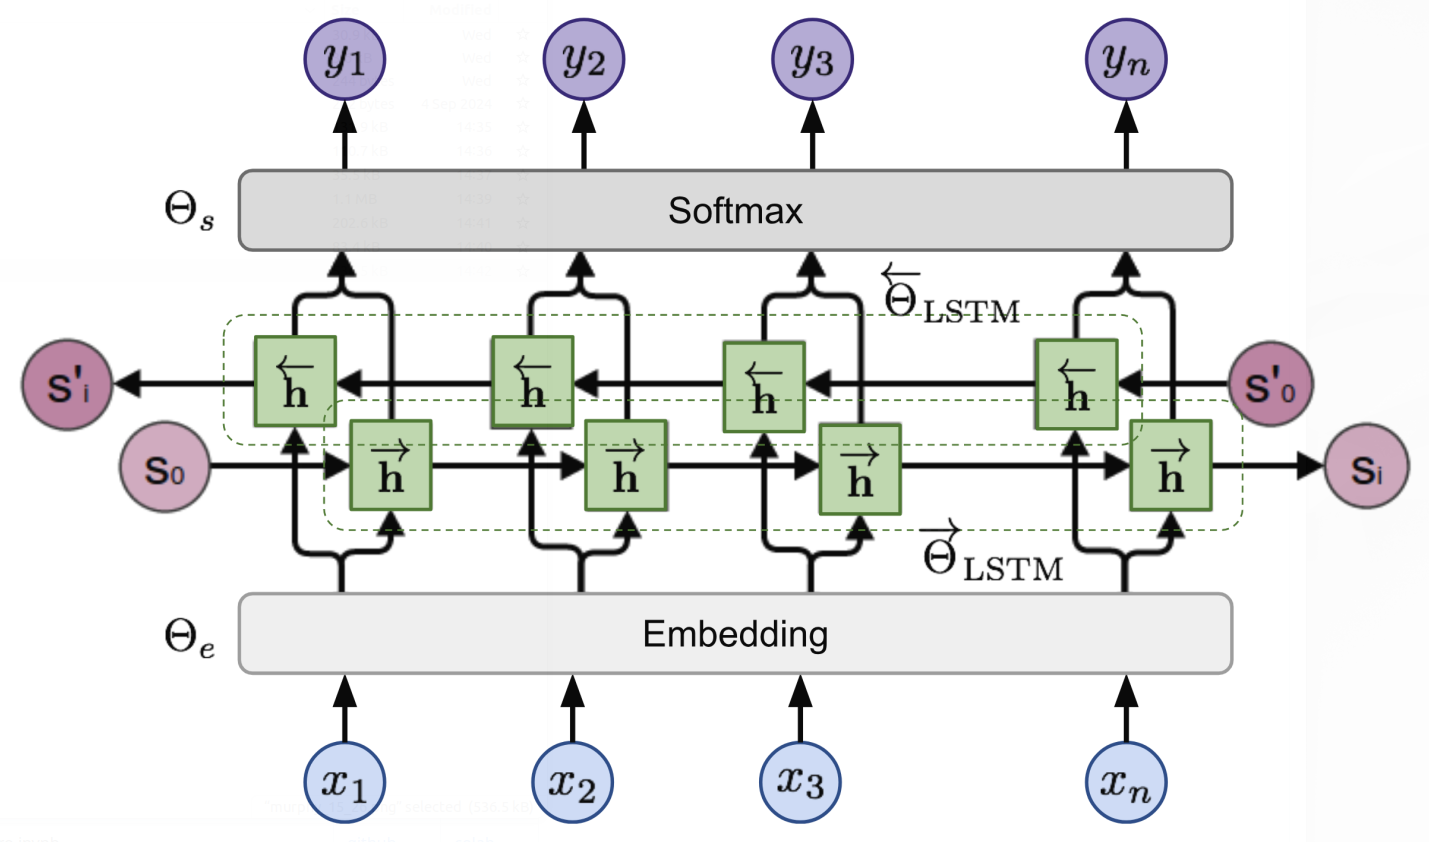
\includegraphics[width=\textwidth]{murphy_15_32.png}
\end{column}
\begin{column}{.2\textwidth}
\scriptsize Source: Murphy, Fig. 15.32 \normalsize
\end{column}
\end{columns}
\end{frame}

\begin{frame}{BERT}
\begin{itemize}
\item  ''Bidirectional Encoder Representations from Transformers''
\item Encoder-only
\item Stacked set of transformers
\item Learns representations of tokens in context of past and future words
\end{itemize}

\textbf{Three embeddings for teach token:}
\begin{center}
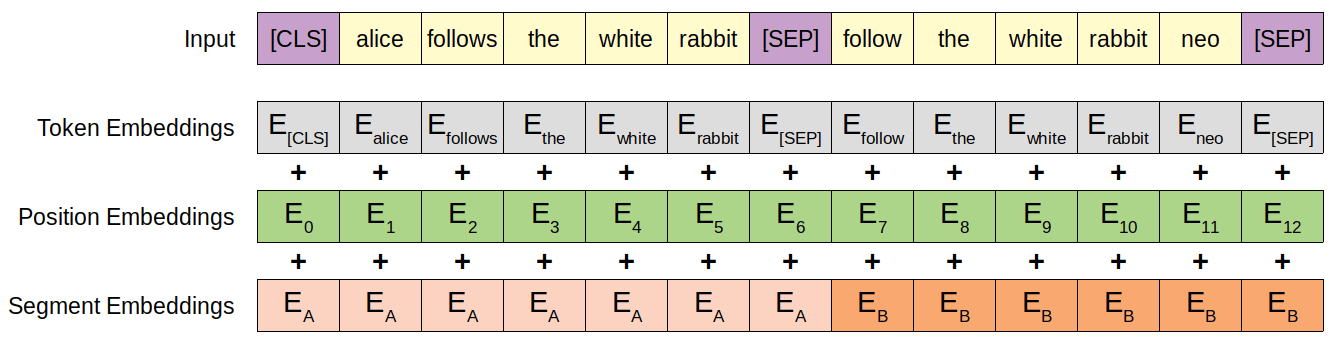
\includegraphics[width=\textwidth]{BERT_input_embeddings.png} \\

\scriptsize \url{https://commons.wikimedia.org/wiki/File:BERT_input_embeddings.png} \normalsize
\end{center}
\end{frame}

\begin{frame}{Comparison of BERT and GPT Architectures}
\centering

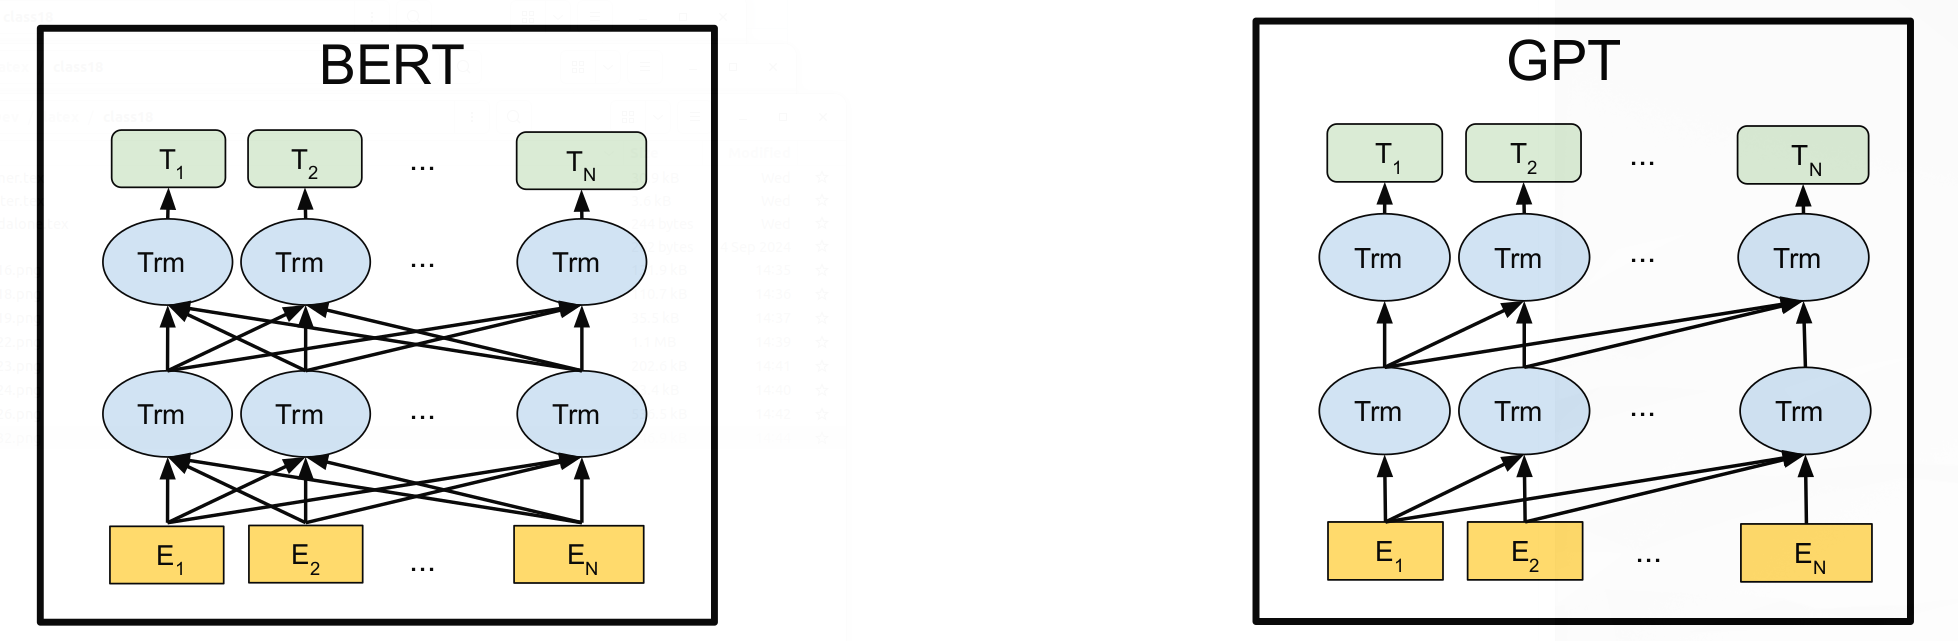
\includegraphics[width=\textwidth]{murphy_15_33.png} \\

\scriptsize Source: Murphy, Fig. 15.33 \normalsize
\end{frame}

\begin{frame}{BERT -- Pre-Training Tasks \small [cont'd]}
\begin{itemize}
   \item Masked Language Modelling
   \item Next sentence prediction
\end{itemize}

\begin{center}
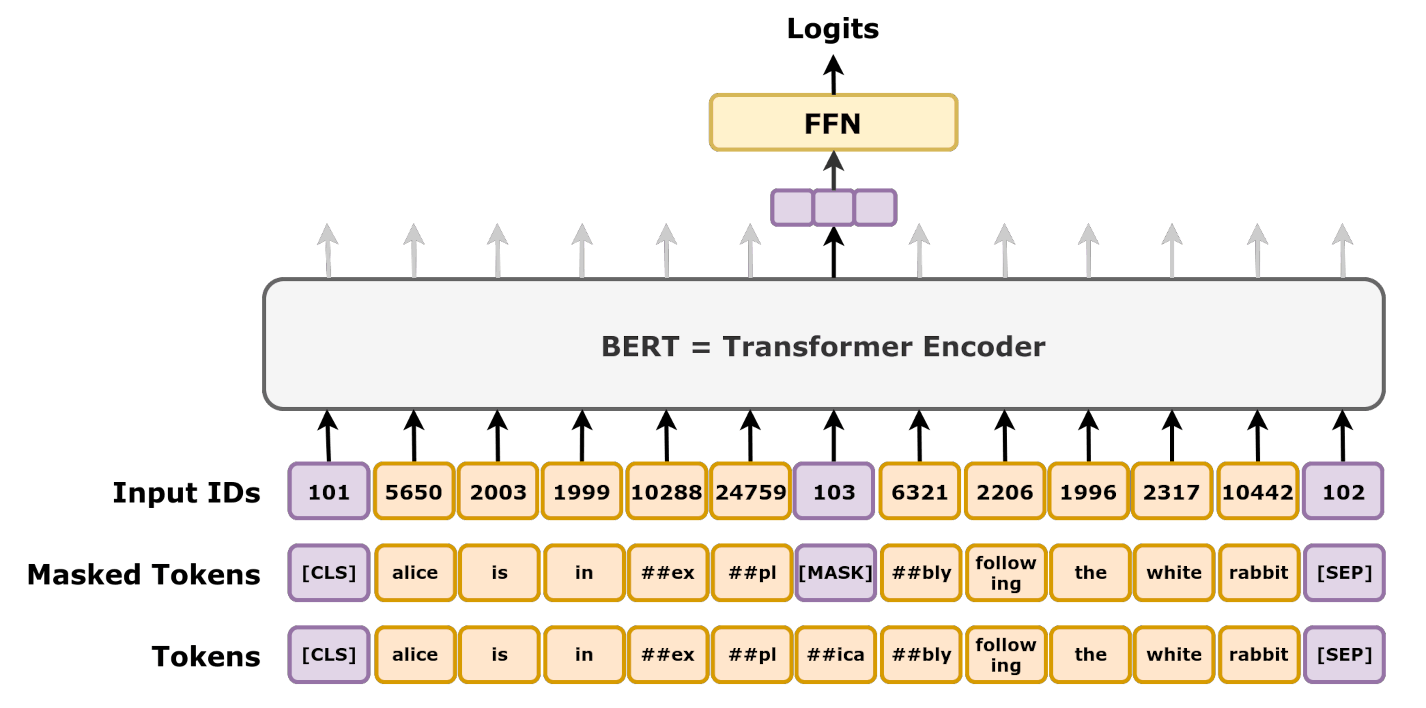
\includegraphics[height=1.15in]{BERT_masked_language_modelling_task.png} \\
\tiny \url{https://commons.wikimedia.org/wiki/File:BERT_masked_language_modelling_task.png} \normalsize \\

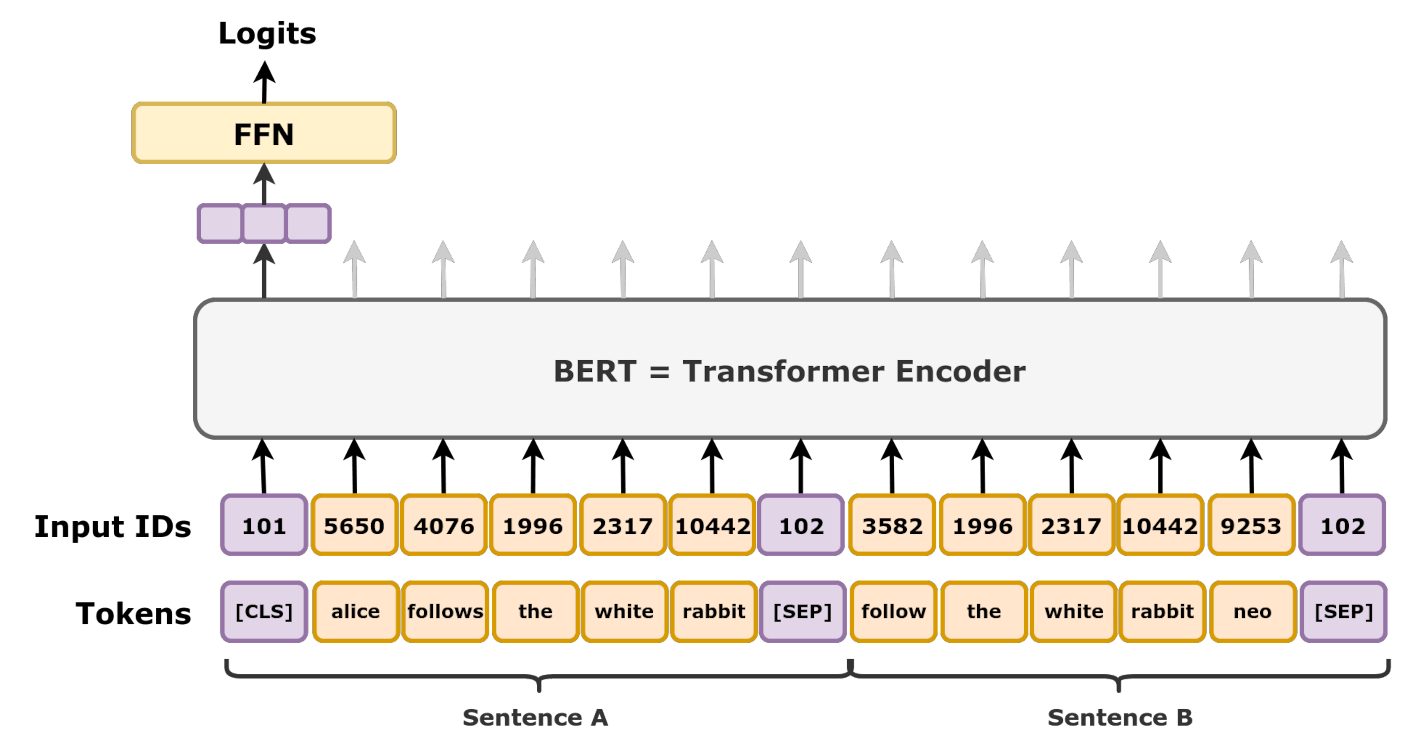
\includegraphics[height=1.15in]{BERT_next_sequence_prediction_task.png} \\
\tiny \url{https://commons.wikimedia.org/wiki/File:BERT_next_sequence_prediction_task.png} \normalsize
\end{center}

\end{frame}

\begin{frame}{BERT -- Example Fine-Tuning Tasks}
\begin{itemize}
   \item Sentence classification
   \item Question answering
   \item Part-of-speech tagging
\end{itemize}

\begin{center}
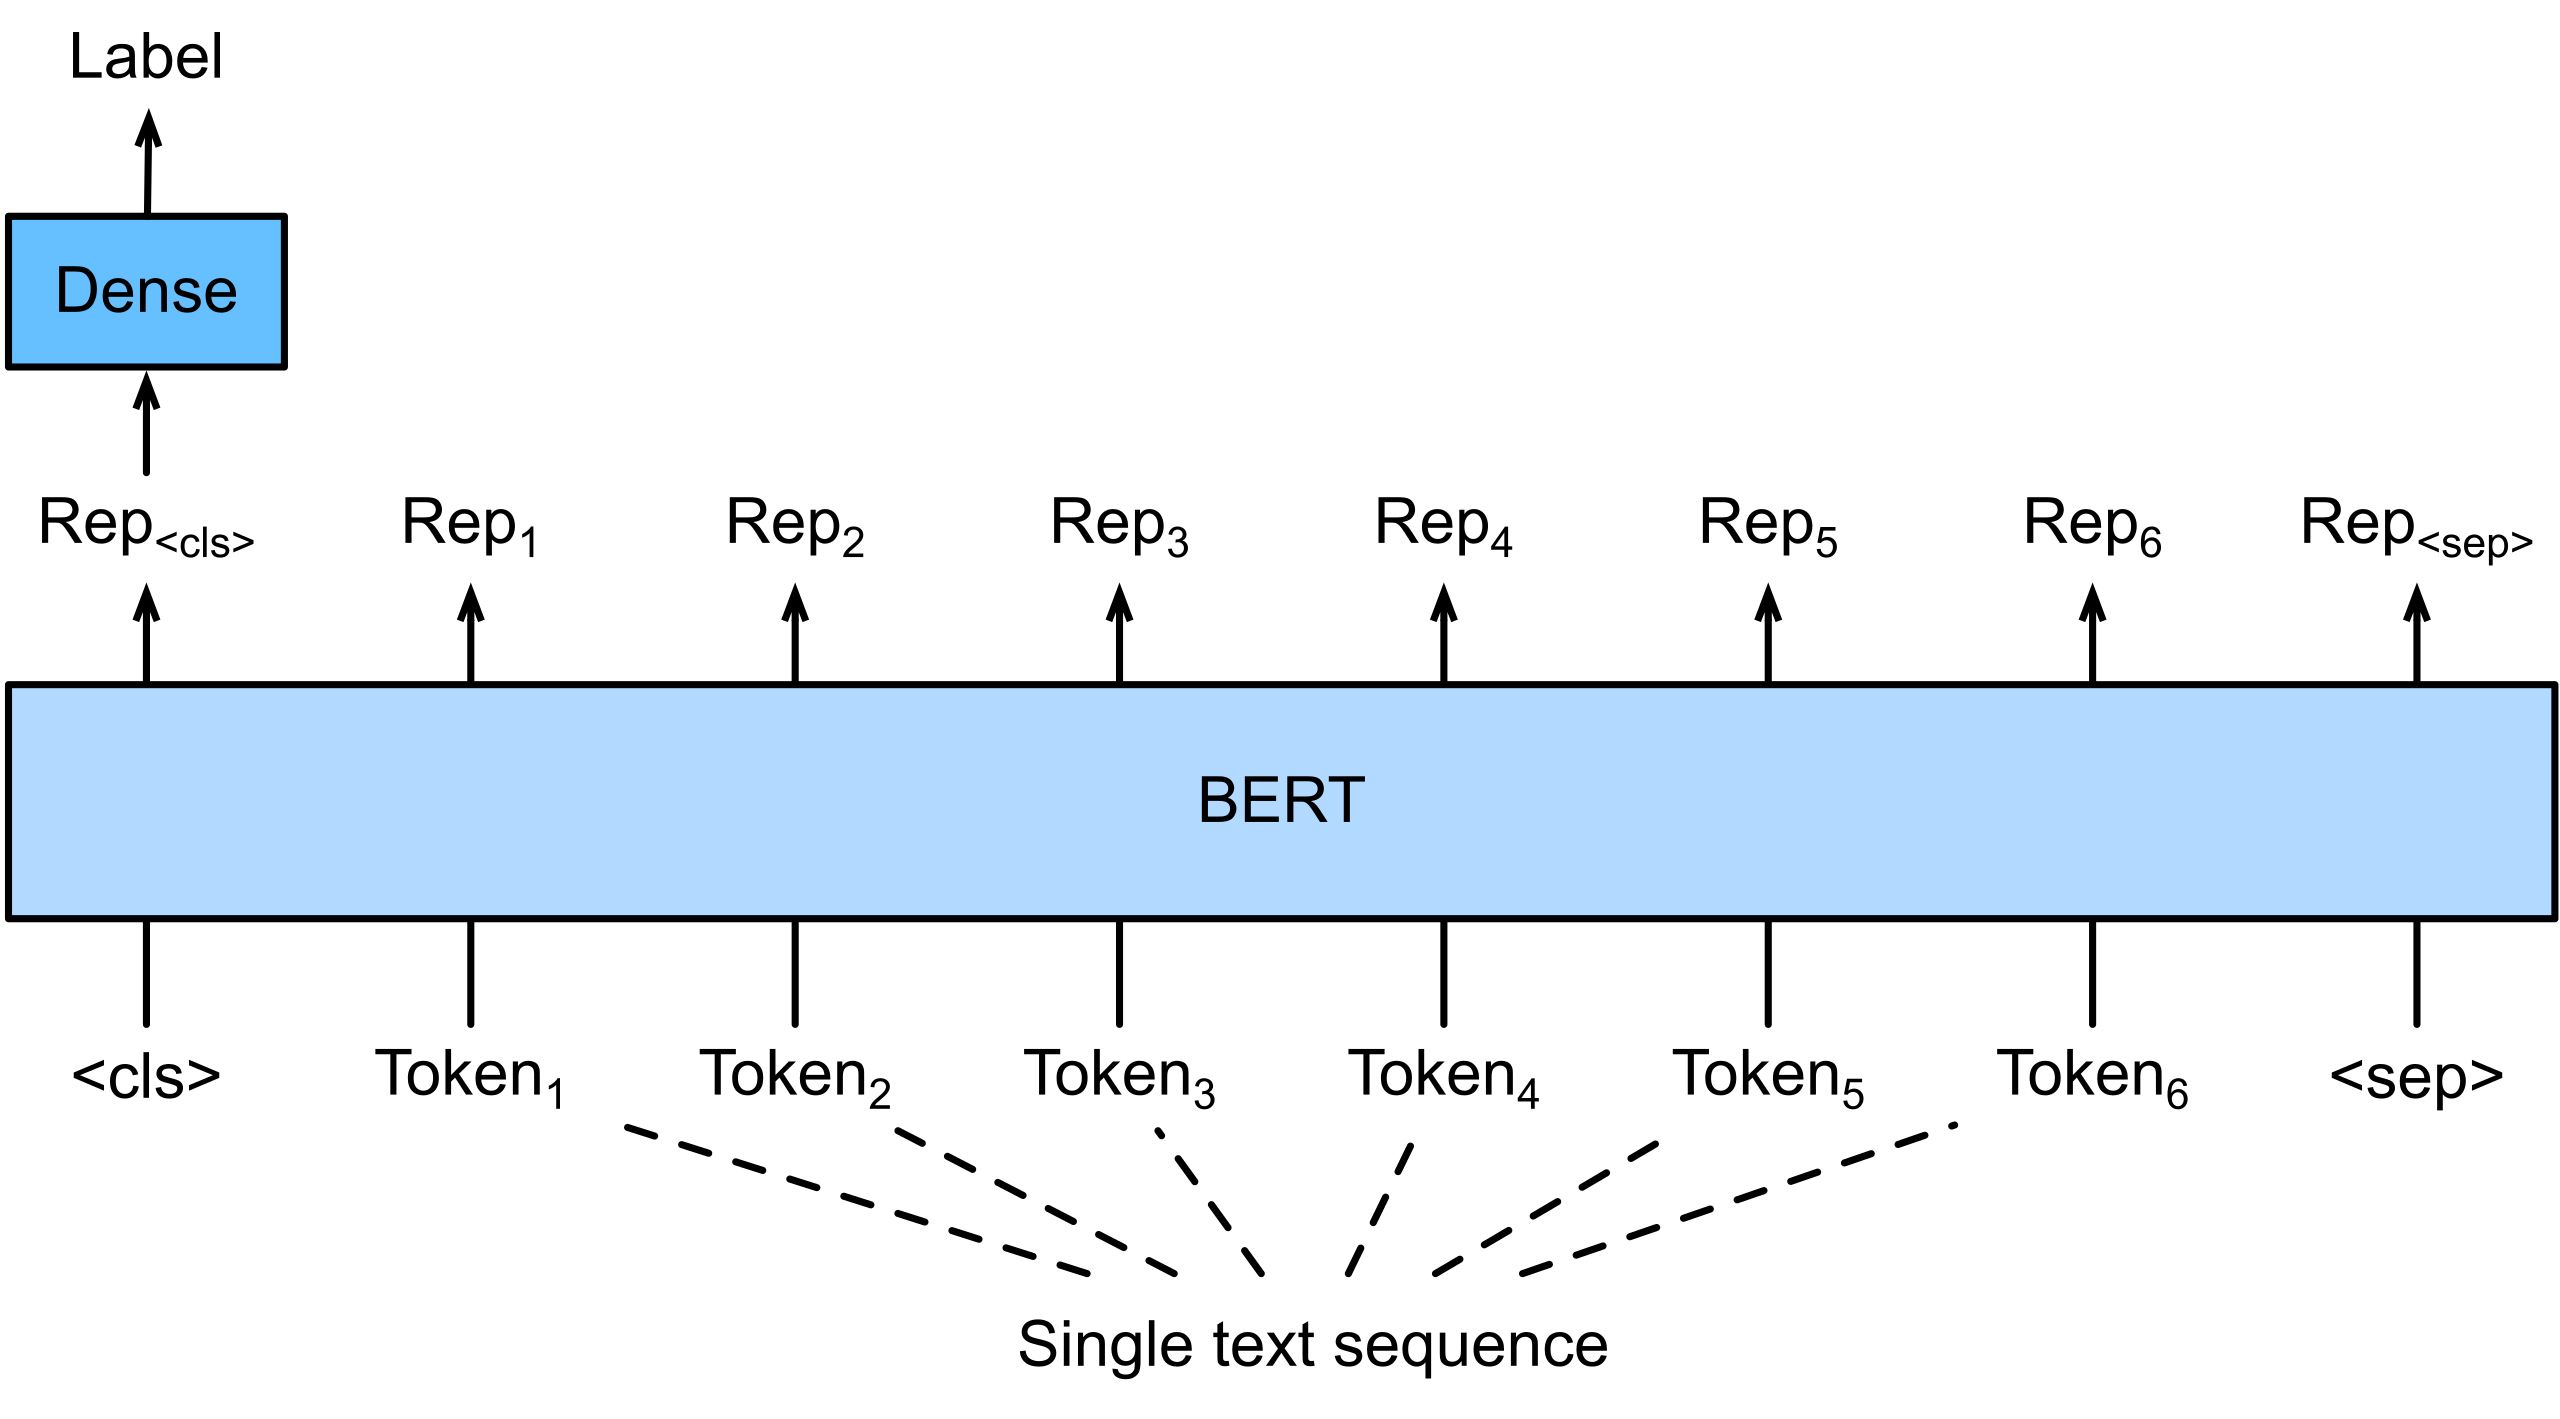
\includegraphics[width=.45\textwidth]{BERT_on_sentence_classification.svg.png} \hspace{.05\textwidth}
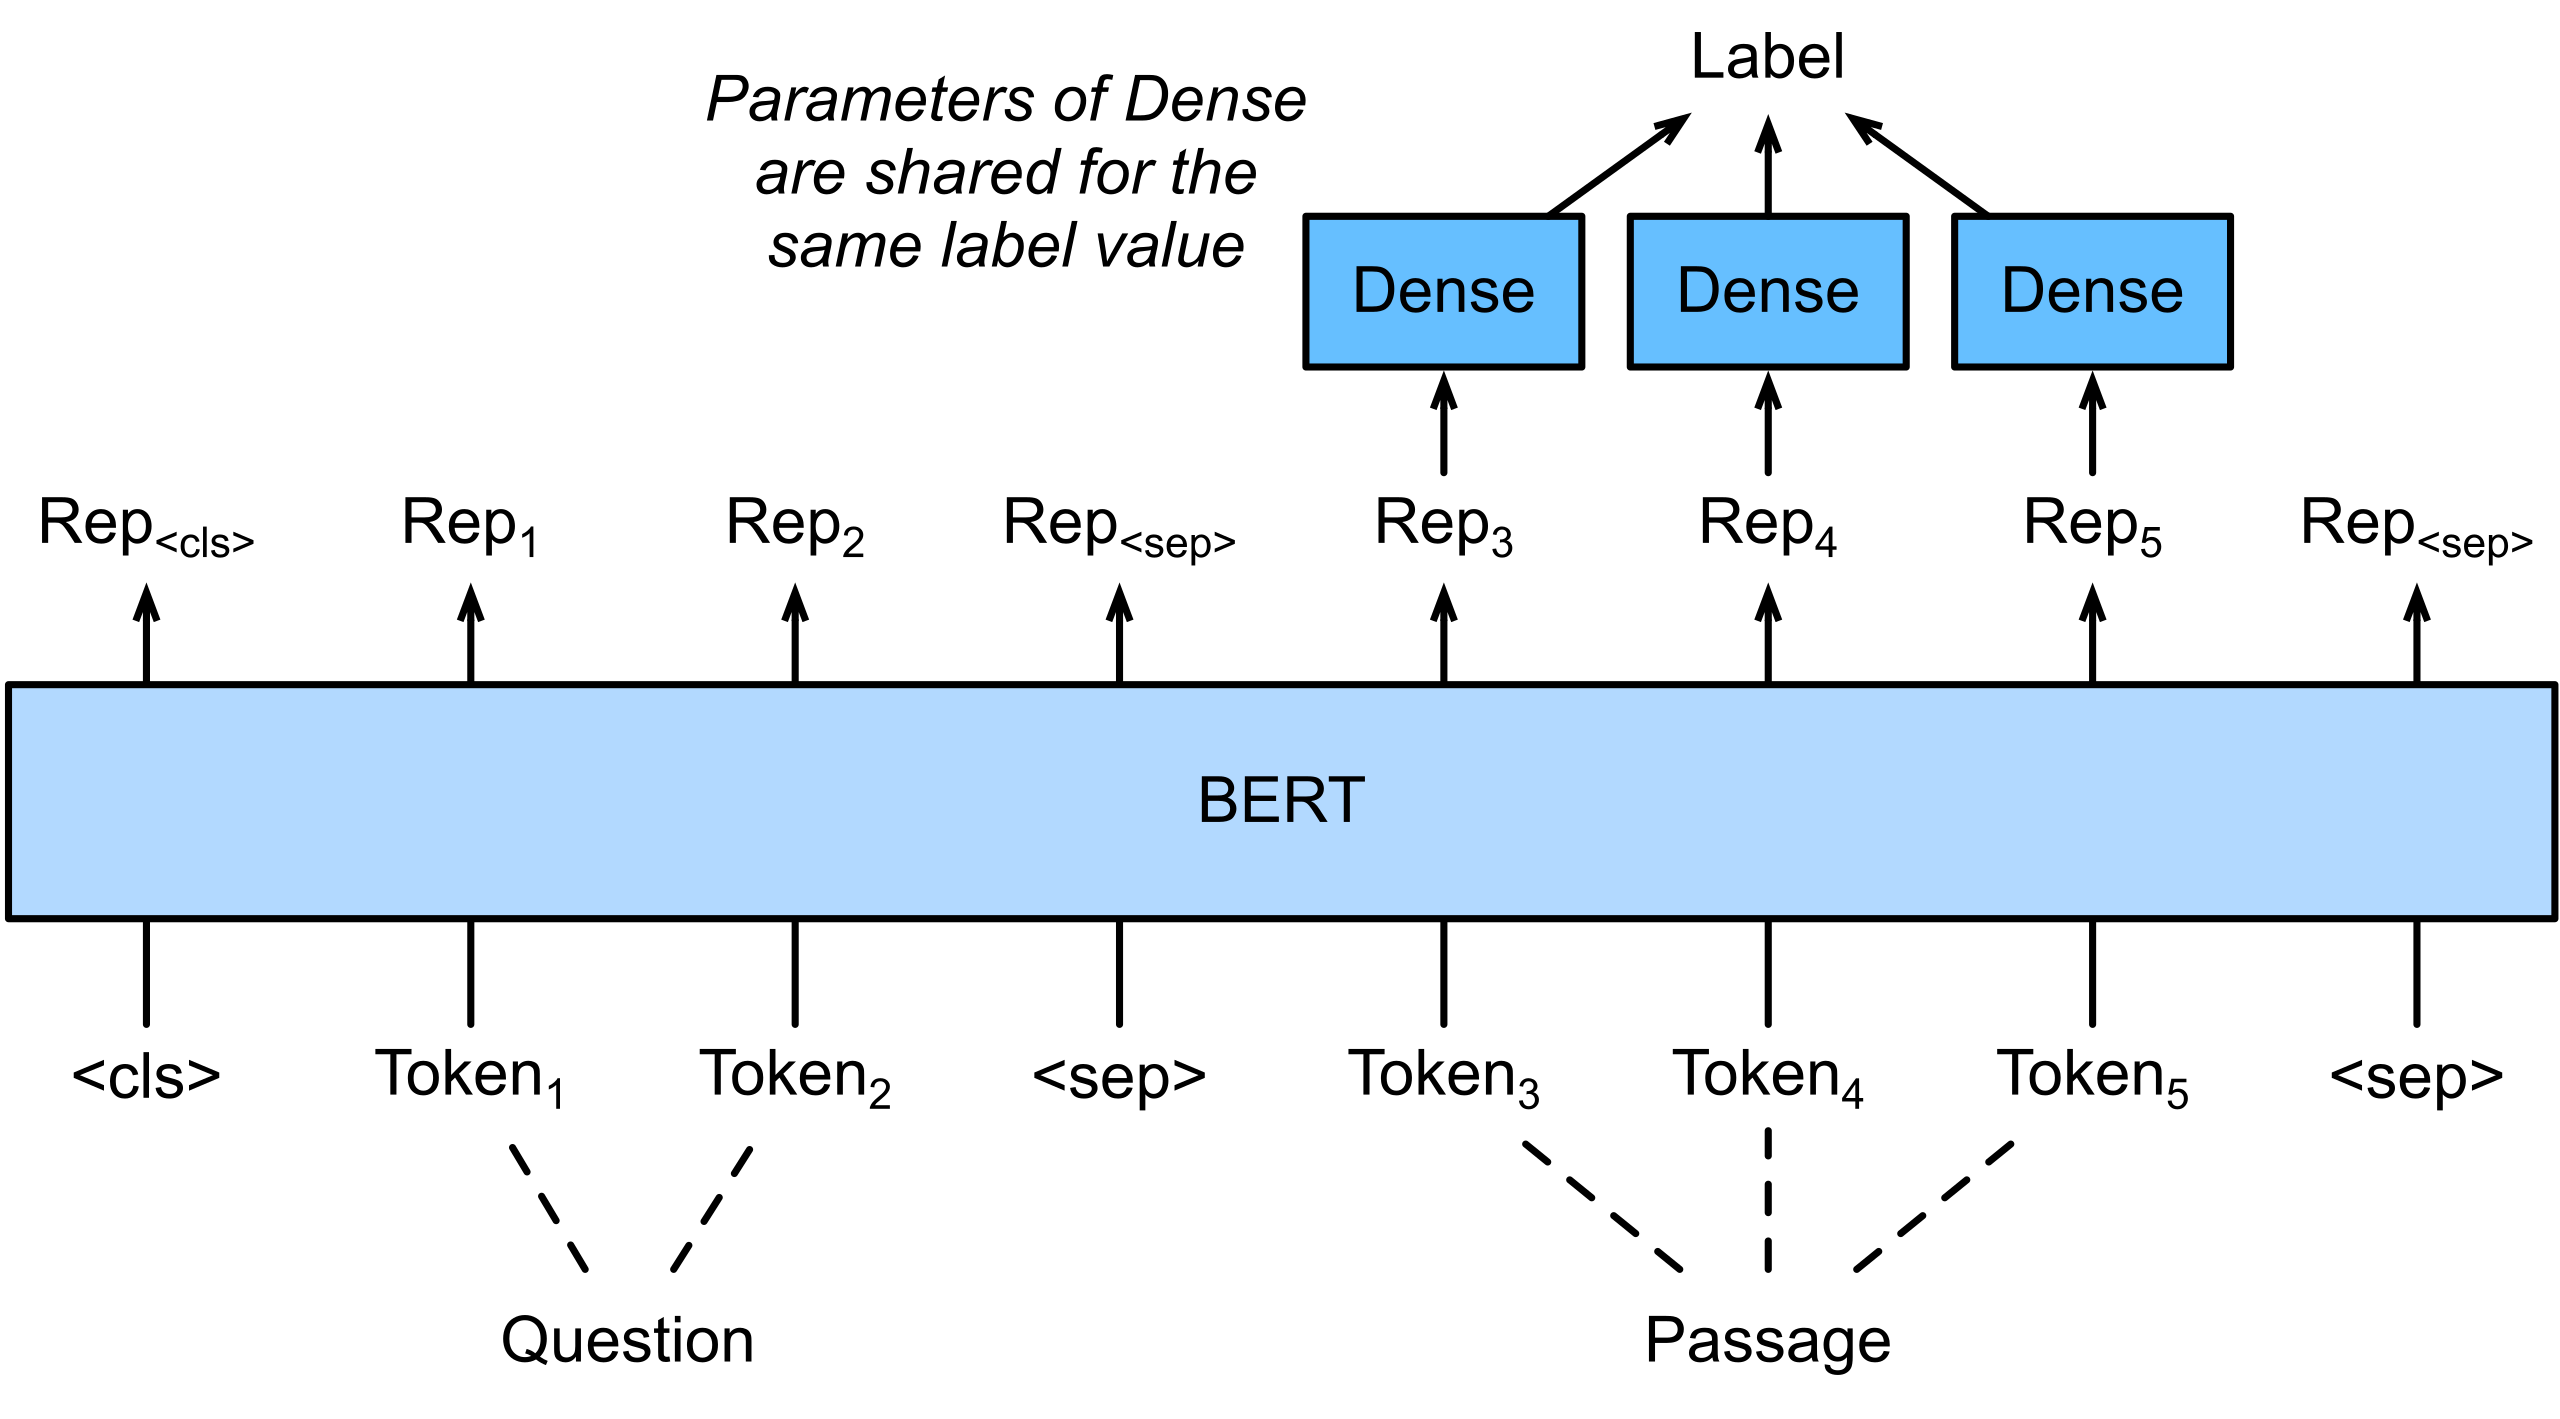
\includegraphics[width=.45\textwidth]{BERT_on_multiple-choice_question-answering.svg.png}
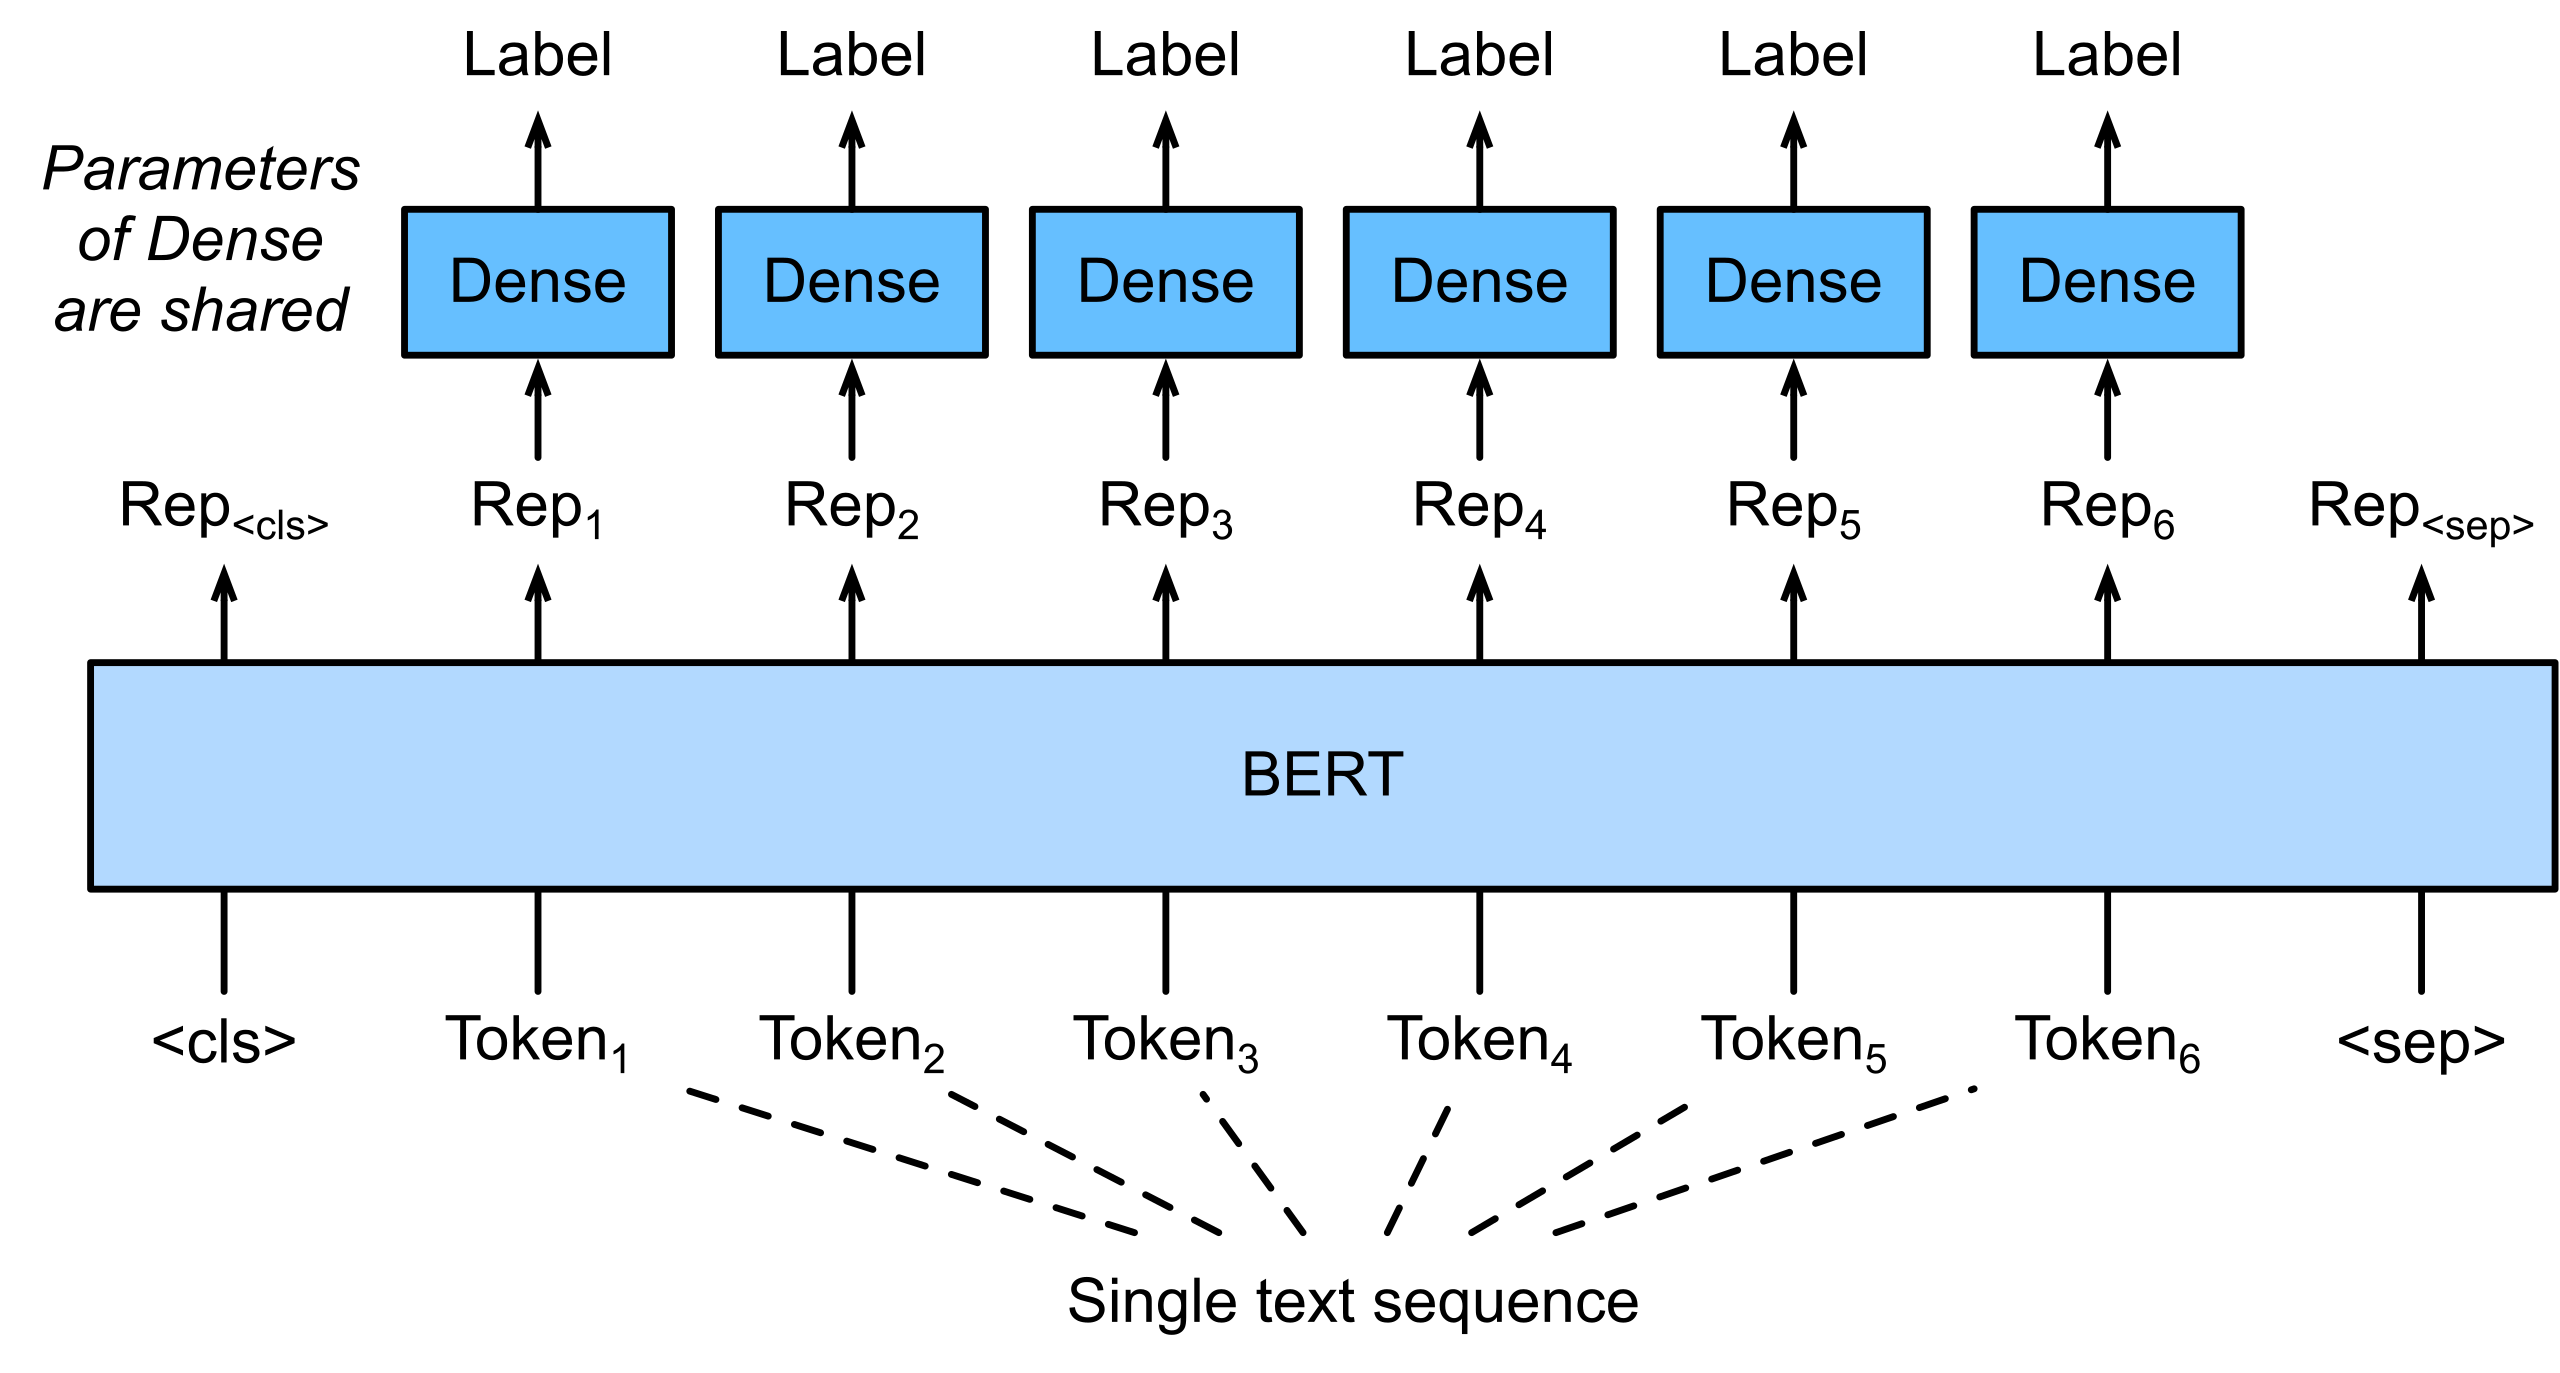
\includegraphics[width=.45\textwidth]{BERT_on_tagging.svg.png}
\end{center}

\tiny
\url{https://commons.wikimedia.org/wiki/File:BERT_on_sentence_classification.svg} \\
\url{https://commons.wikimedia.org/wiki/File:BERT_on_multiple-choice_question-answering.svg} \\
\url{https://commons.wikimedia.org/wiki/File:BERT_on_tagging.svg}

\end{frame}

\begin{frame}{Tensorflow and Keras Tutorials}

\begin{block}{Keras}
\begin{itemize}
\item \href{https://keras.io/examples/generative/text_generation_with_miniature_gpt/}{Text generation with a miniature GPT} 
\item \href{https://keras.io/examples/nlp/text_classification_with_transformer/}{Text classification with a transformer} 
\item \href{https://keras.io/examples/nlp/neural_machine_translation_with_transformer/}{English-to-Spanish translation with seq2seq transformer} 
\item \href{https://keras.io/examples/nlp/semantic_similarity_with_bert/}{Semantic similarity with BERT} 
\end{itemize}
\end{block}

\begin{block}{Tensorflow}
\begin{itemize}
\item \href{https://www.tensorflow.org/text/tutorials/transformer}{Neural machine translation with a Transformer and Keras} 
\item \href{https://www.tensorflow.org/text/tutorials/classify_text_with_bert}{Classify text with BERT} 
\item \href{https://www.tensorflow.org/tfmodels/nlp/fine_tune_bert}{Fine-tuning a BERT model} 
\end{itemize}
\end{block}
\end{frame}

\begin{frame}{Auto-Encoder}

Map input to \emph{point} in lower-dimensional latent space:

\begin{columns}
\begin{column}{.5\textwidth}
\begin{center}
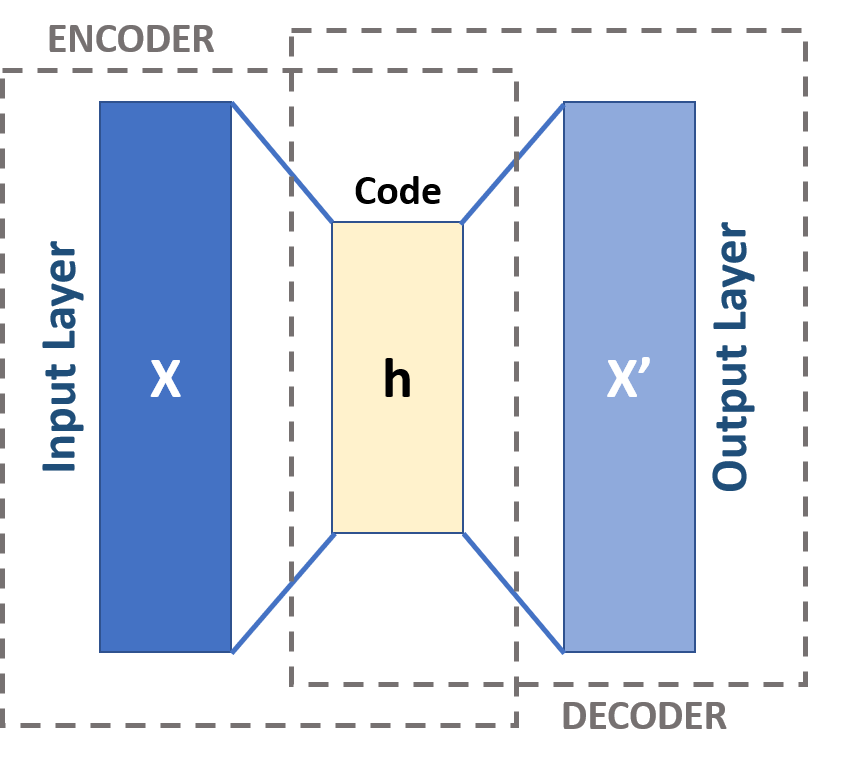
\includegraphics[height=1.5in]{Autoencoder_schema.png}
\end{center}
\end{column}
\begin{column}{.4\textwidth}
\scriptsize \url{https://commons.wikimedia.org/wiki/File:Autoencoder_schema.png} \normalsize
\end{column}
\end{columns}

\begin{block}{Usage}
\begin{itemize}
   \item Face recognition
   \item Feature detection
   \item Anomaly detection
   \item Data synthesis (by adding noise to points in latent space)
\end{itemize}
\end{block}
\end{frame}
   
\begin{frame}{Auto-Encoder Examples}
\textbf{Fashion MNIST -- Original and Reconstruction}
\begin{itemize}
   \item \emph{Left:} 3-layer densely connected network (decoder inverse)
   \item \emph{Right:} 3-layer CNN (decoder inverse)
\end{itemize} 

\begin{center}
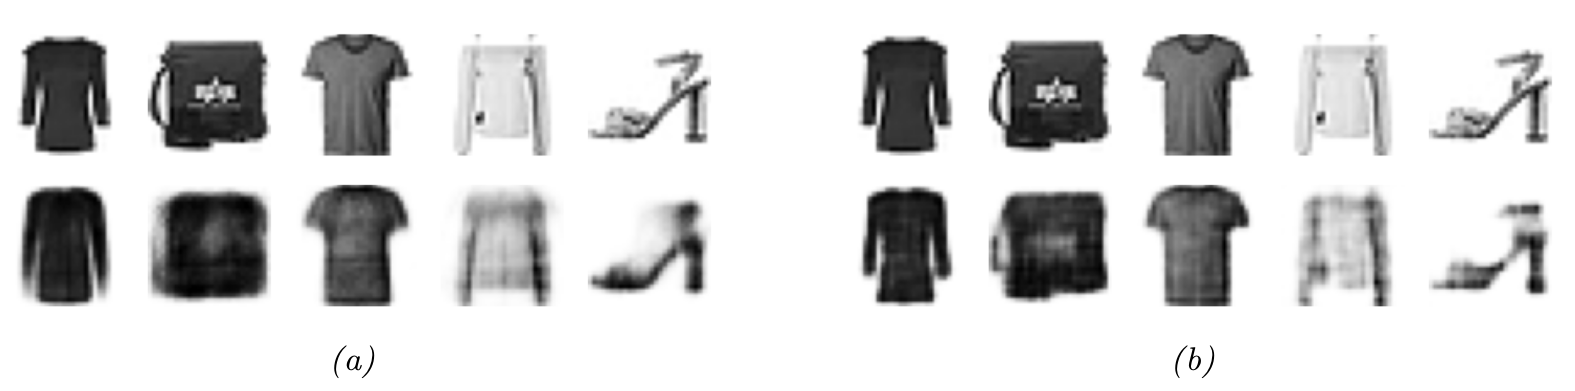
\includegraphics[width=\textwidth]{murphy_20_17.png} \\

\scriptsize Source: Murphy, Fig. 20.17 \normalsize
\end{center}
\end{frame}

\begin{frame}{Auto-Encoder Examples}
\textbf{Fashion MNIST -- First 2 Latent Dimensions}
\begin{itemize}
   \item \emph{Left:} 3-layer densely connected network (decoder inverse)
   \item \emph{Right:} 3-layer CNN (decoder inverse)
\end{itemize} 

\begin{center}
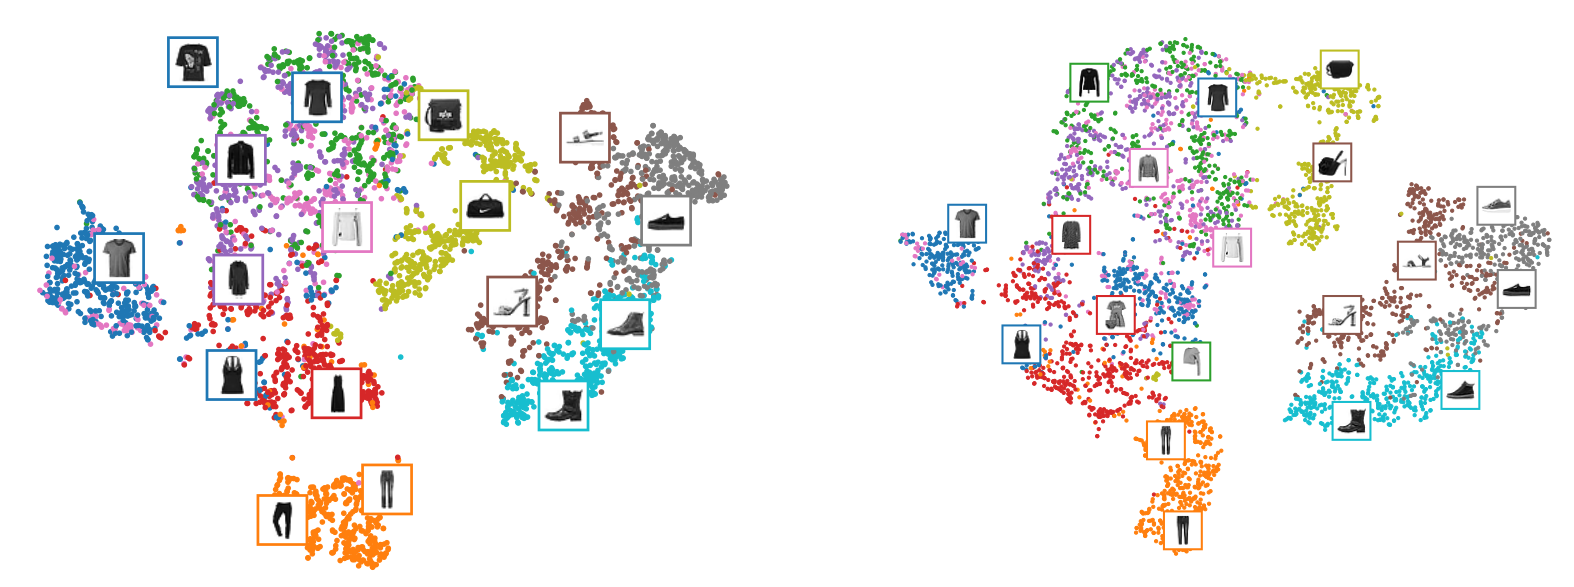
\includegraphics[width=\textwidth]{murphy_20_18.png} \\

\scriptsize Source: Murphy, Fig. 20.18 \normalsize
\end{center}
\end{frame}

\begin{frame}{Auto-Encoder in Python}

Implementations are available on the following GitHub repo:

\url{https://github.com/jevermann/busi4720-ai} \\


The project can be cloned from this URL:

\url{https://github.com/jevermann/busi4720-ai.git}

\begin{block}{Important}
While the encoder and decoder in the following examples have the same architecture, this need not be the case! One could encode with a CNN and decode with a dense network, or any other combination of architectures.
\end{block}

\end{frame}

\begin{frame}[fragile]{Auto-Encoder in Python \small [cont']}
Encoder:
\begin{pythoncode}
from tensorflow.keras import layers
from tensorflow.keras import models
import keras

encoder = models.Sequential([
    layers.Flatten(),
    layers.Dense(1000),
    layers.Dropout(0.25),
    layers.Dense(500),
    layers.Dropout(0.25),
    layers.Dense(30)
])
\end{pythoncode}
Decoder:
\begin{pythoncode}
decoder = models.Sequential([
    layers.Dense(500),
    layers.Dense(1000),
    layers.Dense(28*28),
    layers.Reshape(target_shape=(28, 28))
])
\end{pythoncode}
\end{frame}

\begin{frame}[fragile]{Auto-Encoder in Python \small [cont']}
Complete auto-encoder model:

\begin{pythoncode}
auto_encoder = models.Sequential([encoder, decoder])
\end{pythoncode}

Load and transform data:
\begin{pythoncode}
(x_train, y_train), (x_test, y_test) = \
                    keras.datasets.fashion_mnist.load_data()
x_train = x_train / 255.0
x_test = x_test / 255.0
\end{pythoncode}

Compile and train the auto-encoder:
\begin{pythoncode}
auto_encoder.compile(loss="mse")
auto_encoder.fit(x_train, x_train, 
                 epochs=5, validation_data=(x_test, x_test))
\end{pythoncode}
\end{frame}

\begin{frame}[fragile]{CNN Auto-Encoder in Python \small [cont']}

Encoder:
\begin{pythoncode}
encoder = models.Sequential([
    layers.Reshape([28, 28, 1], input_shape=[28, 28]),
    layers.Conv2D(16, (3, 3), 
                  padding="same", activation="relu"),
    layers.MaxPool2D((2, 2)),
    layers.Conv2D(32, (3, 3), 
                  padding="same", activation="relu"),
    layers.MaxPool2D((2, 2)),
    layers.Conv2D(64, (3, 3), 
                  padding="same", activation="relu"),
    layers.MaxPool2D((2, 2))])
\end{pythoncode}

Decoder:
\begin{pythoncode}
decoder = models.Sequential([
    layers.Conv2DTranspose(32, (3, 3), strides=2, 
               activation="relu", input_shape=[3, 3, 64]),
    layers.Conv2DTranspose(16, (3, 3), strides=2, 
               padding="same", activation="relu"),
    layers.Conv2DTranspose(1, (3, 3), strides=2, 
               padding="same", activation="sigmoid"),
    layers.Reshape([28, 28])])
\end{pythoncode}
\end{frame}


\begin{frame}{Auto-Encoder -- Denoising}
\begin{itemize}
   \item Add noise to input
   \item Reconstruct clean output
   \item Reconstruction/recognition of ''corrupted'' images
\end{itemize}
 
\begin{center}
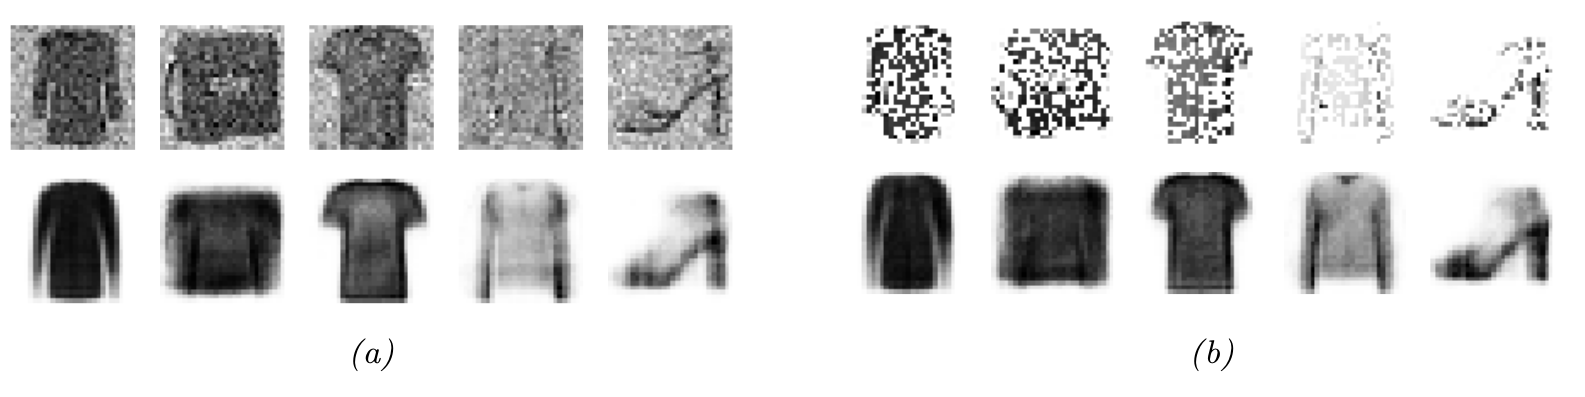
\includegraphics[width=\textwidth]{murphy_20_19.png} \\

\scriptsize Source: Murphy, Fig. 20.19 \normalsize
\end{center}
\end{frame}
   

\begin{frame}{VAE -- Variational Auto-Encoder}

\begin{columns}
\begin{column}{.5\textwidth}
\begin{center}
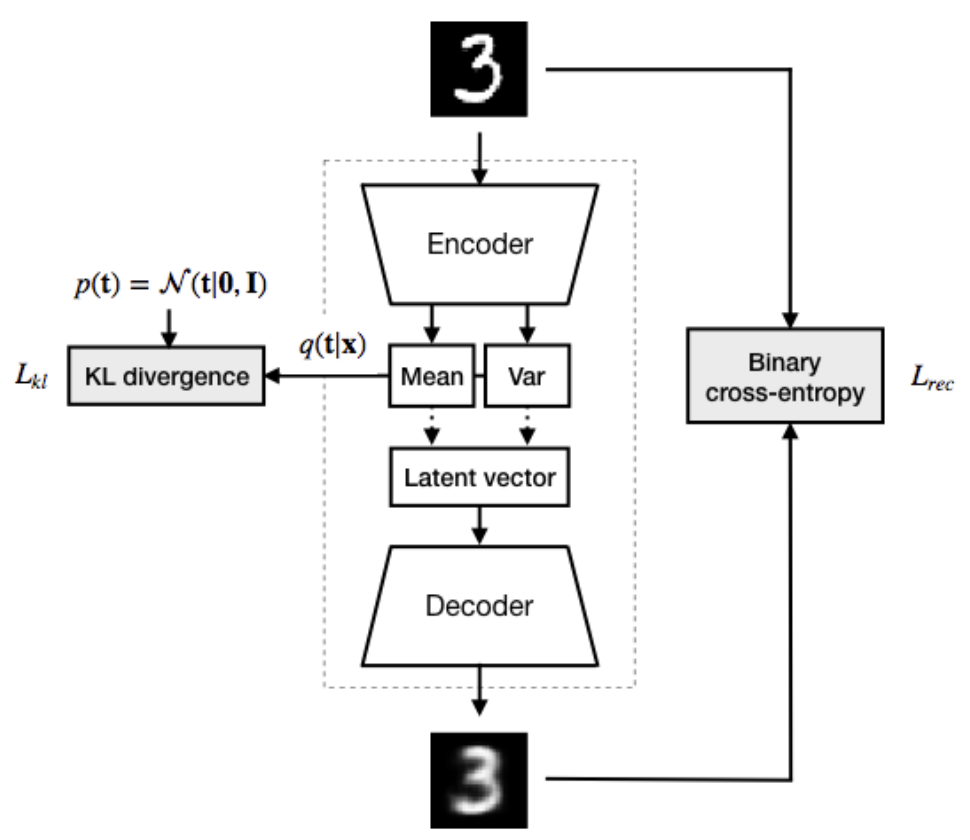
\includegraphics[height=2in]{murphy_20_22.png}\\

\scriptsize Source: Murphy, Fig. 20.22 \normalsize \\
\end{center}

%\vspace{\baselineskip}
%\small
\textbf{Example:} Map into Gaussian with mean vector $\mu$ and covariance matrix $\Sigma$
\end{column}
\begin{column}{.5\textwidth}
\begin{block}{Principles}
%\small
\begin{itemize}
\item Map input to \emph{probability distribution} in lower - dimensional latent space.
\item Sample a point in latent space from that distribution
\item Loss is reconstruction loss plus (KL) distribution divergence loss, e.g. from normal
\end{itemize}
\end{block}
\end{column}
\end{columns}
\end{frame}

   
\begin{frame}{VAE -- Variational Auto-Encoder}

\begin{itemize}

\item Training and Reparameterization:

\begin{center}
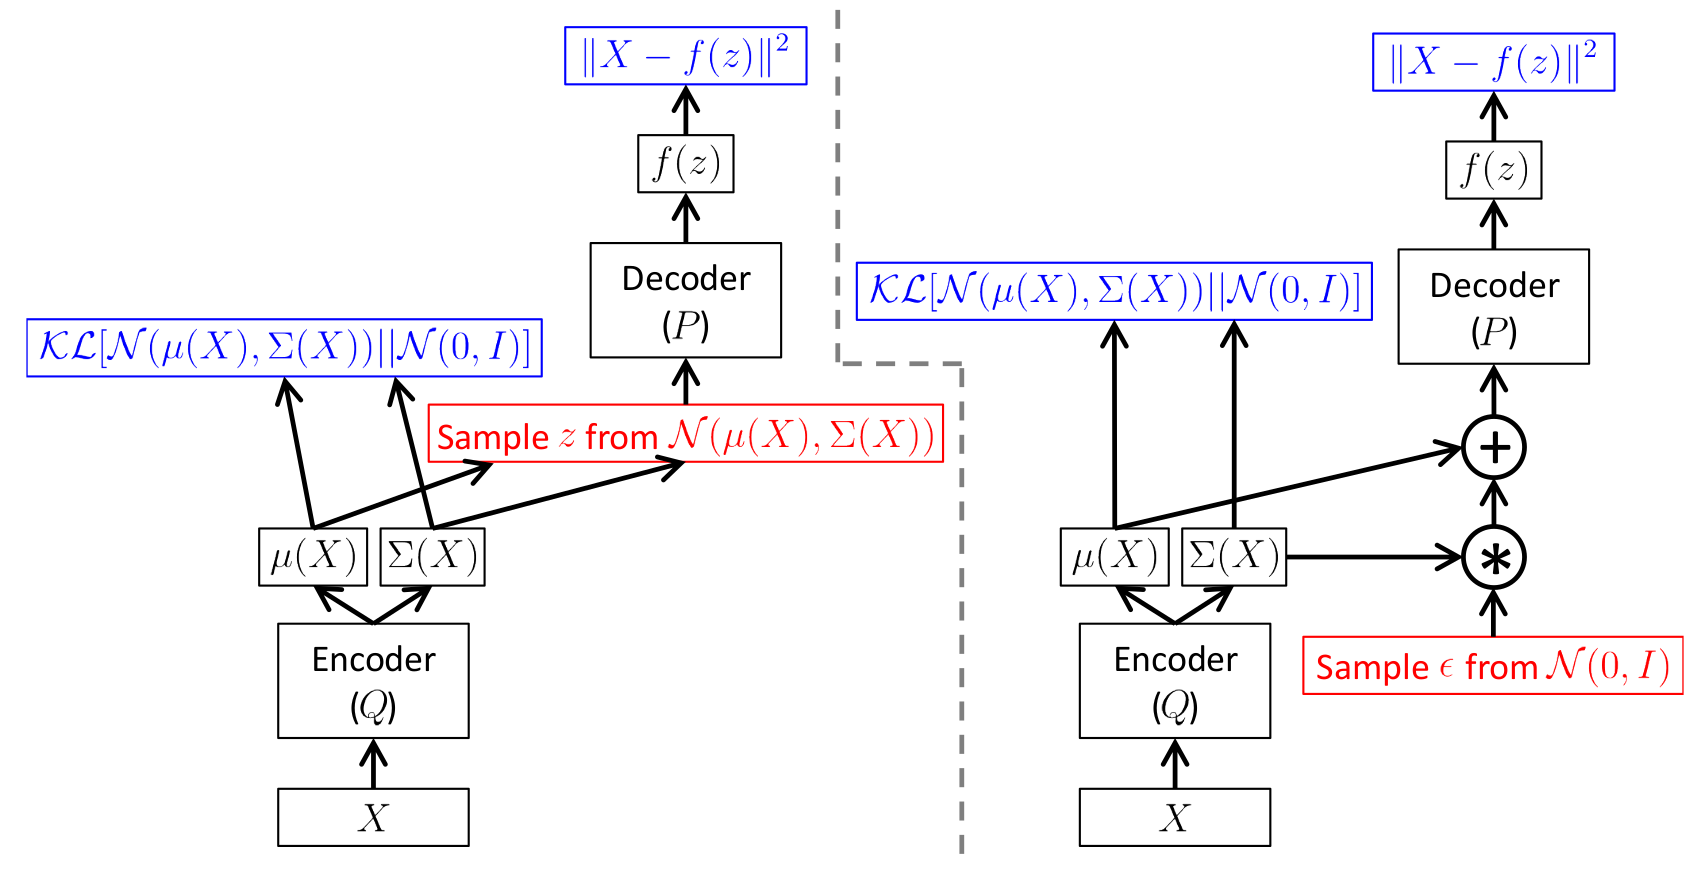
\includegraphics[width=.8\textwidth]{murphy_20_23.png}\\

\scriptsize Source: Murphy, Fig. 20.23 \normalsize
\end{center}

\item Ensures contiguous use of latent space
\item Allows generation by sampling from a Gaussian and decoding (in contrast to deterministic AE)
\end{itemize}

\end{frame}

\begin{frame}{VAE -- Variational Auto-Encoder}

Reconstruction: VAE (a) --- AE (b) \\
\begin{center}
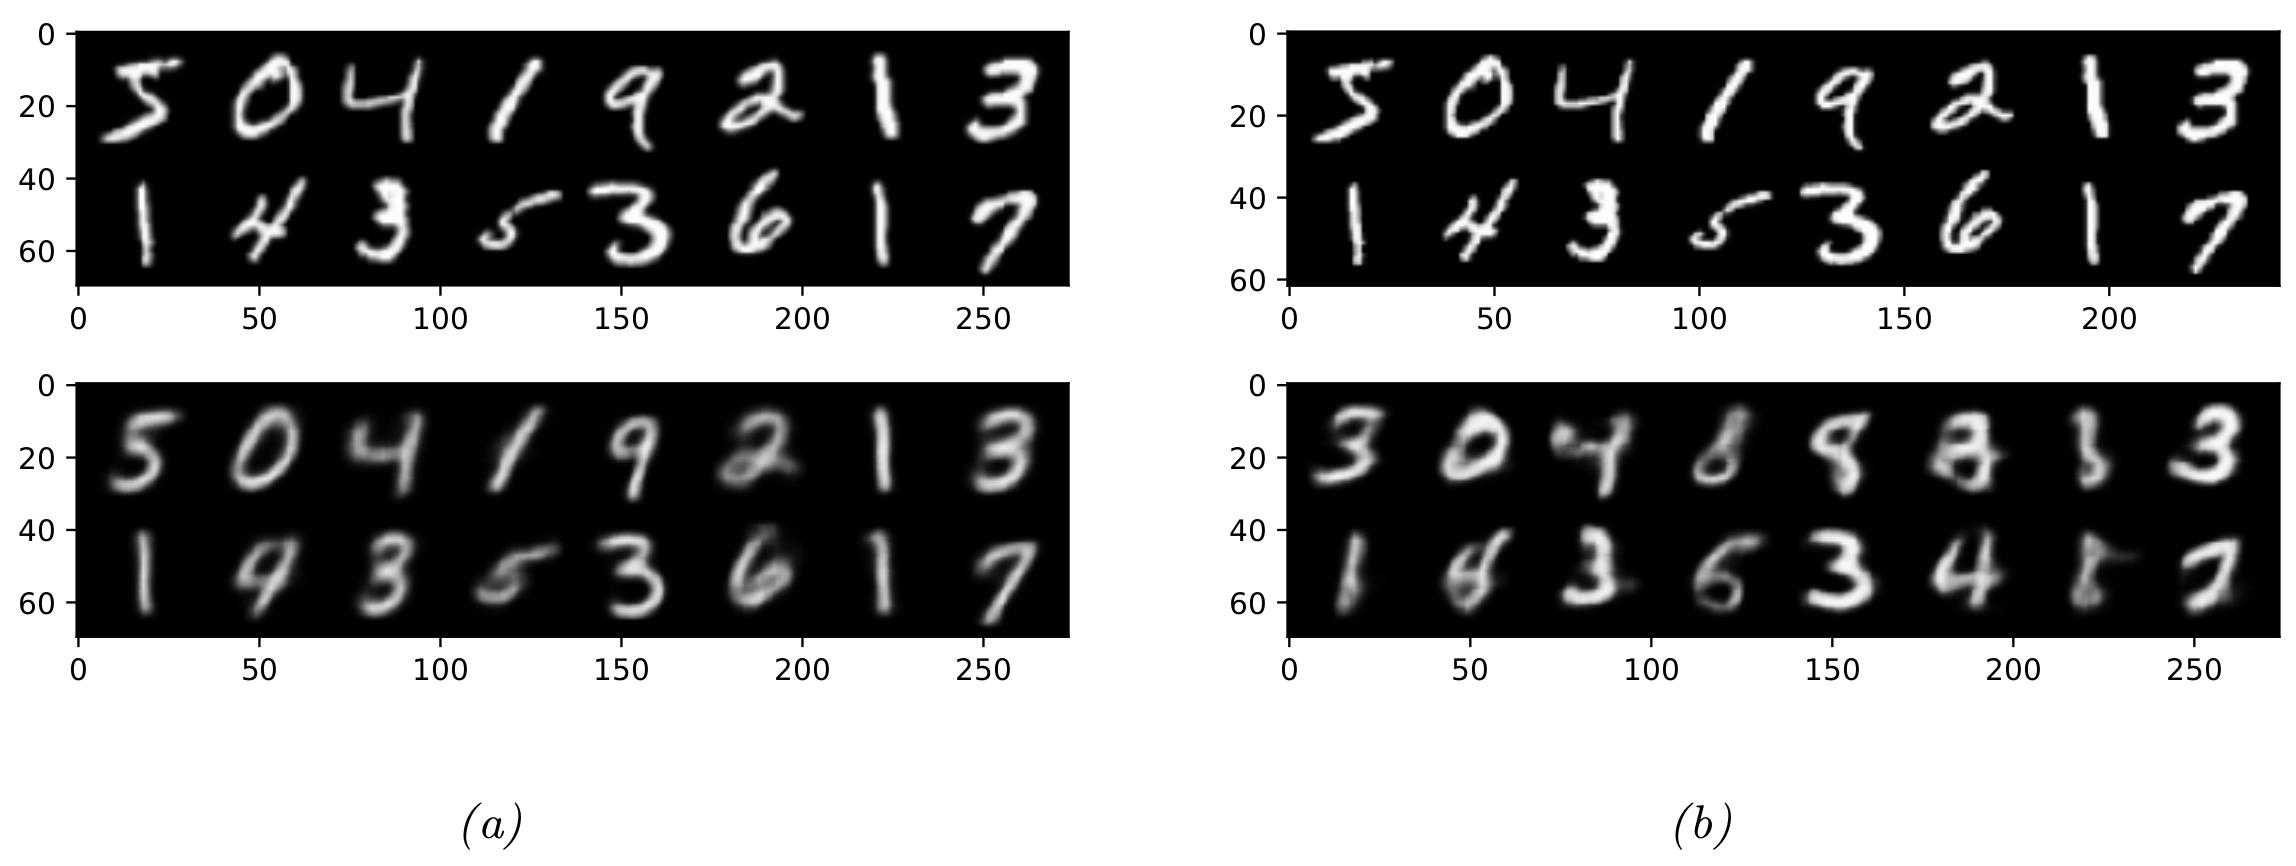
\includegraphics[width=.8\textwidth]{murphy_20_24.png} \\
\scriptsize Source: Murphy Fig. 20.24 \normalsize
\end{center}

Generation: VAE (a) --- AE (b) \\
\begin{center}
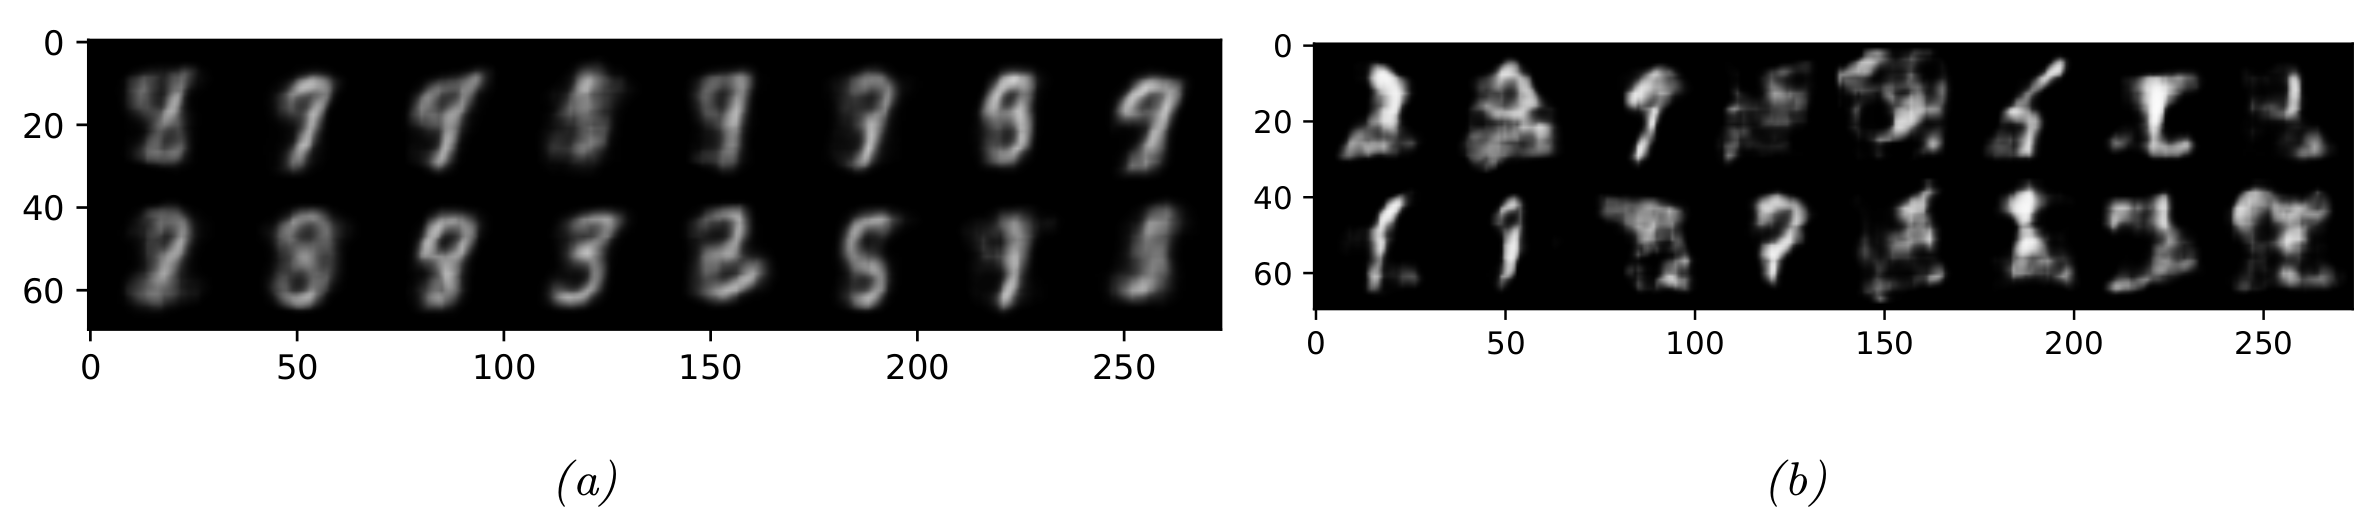
\includegraphics[width=.8\textwidth]{murphy_20_25.png} \\
\scriptsize Source: Murphy Fig. 20.25 \normalsize
\end{center}
\end{frame}

\begin{frame}{VAE in Python}

Adapted from: 

\small\url{https://keras.io/examples/generative/vae/}\normalsize \\

Implementation available on the following GitHub repo:

\small\url{https://github.com/jevermann/busi4720-ai}\normalsize \\

The project can be cloned from this URL:

\small\url{https://github.com/jevermann/busi4720-ai.git}\normalsize
\end{frame}


\begin{frame}[fragile]{VAE in Python \small [cont']}

Sampling layer for sampling from a multi-variate Gaussian with given mean and log-variance vectors:
\begin{pythoncode}
import tensorflow as tf
import keras
from tensorflow.keras import layers

class Sampling(layers.Layer):
    def call(self, inputs):
        z_mean, z_log_var = inputs
        batch = tf.shape(z_mean)[0]
        dim = tf.shape(z_mean)[1]
        epsilon = tf.random.normal(shape=(batch, dim))
        return z_mean + tf.exp(0.5 * z_log_var) * epsilon
\end{pythoncode}
\end{frame}

\begin{frame}[fragile]{VAE in Python \small [cont'd]}

Encoder:

\begin{pythoncode}
# This is NOT a sequential model
encoder_inputs = tf.keras.Input(shape=(28, 28, 1))
x = layers.Conv2D(32, (3,3), activation="relu", 
             strides=2, padding="same")(encoder_inputs)
x = layers.Conv2D(64, (3,3), activation="relu", 
             strides=2, padding="same")(x)
x = layers.Flatten()(x)
x = layers.Dense(16, activation="relu")(x)

# Vector of means
z_mean = layers.Dense(10, name="z_mean")(x)

# Vector of log variances
z_log_var = layers.Dense(10, name="z_log_var")(x)

# Point in latent space
z = Sampling()([z_mean, z_log_var])

encoder = keras.Model(encoder_inputs, [z_mean, z_log_var, z])
\end{pythoncode}
\end{frame}

\begin{frame}[fragile]{VAE in Python \small [cont'd]}
Loss function:

\begin{pythoncode}
    def vae_loss(encoder, decoder, data):
        z_mean, z_log_var, z = encoder(data)
        reconstruction = decoder(z)
        mse_loss = keras.losses.MeanSquaredError()
        reconstruction_loss = mse_loss(data, reconstruction)
        kl_loss = -0.5 * (1 +
                          z_log_var -
                          tf.square(z_mean) -
                          tf.exp(z_log_var))
        kl_loss = tf.reduce_mean(tf.reduce_sum(kl_loss,axis=1))
        total_loss = reconstruction_loss + kl_loss
        return total_loss
\end{pythoncode}

\begin{itemize}
\item Combination of reconstruction loss and KL loss (''difference'' to standard normal distribution)
\end{itemize}
\end{frame}

\begin{frame}{GAN -- Generative Adversarial Networks}

\begin{itemize}

\item Generator produces data from a latent representation
\item Discriminator attempts to distinguish generated output and true data
\item Generator is trained to generate data that discriminator classifies as real
\end{itemize}

\begin{columns}
\begin{column}{.6\textwidth}
\begin{center}
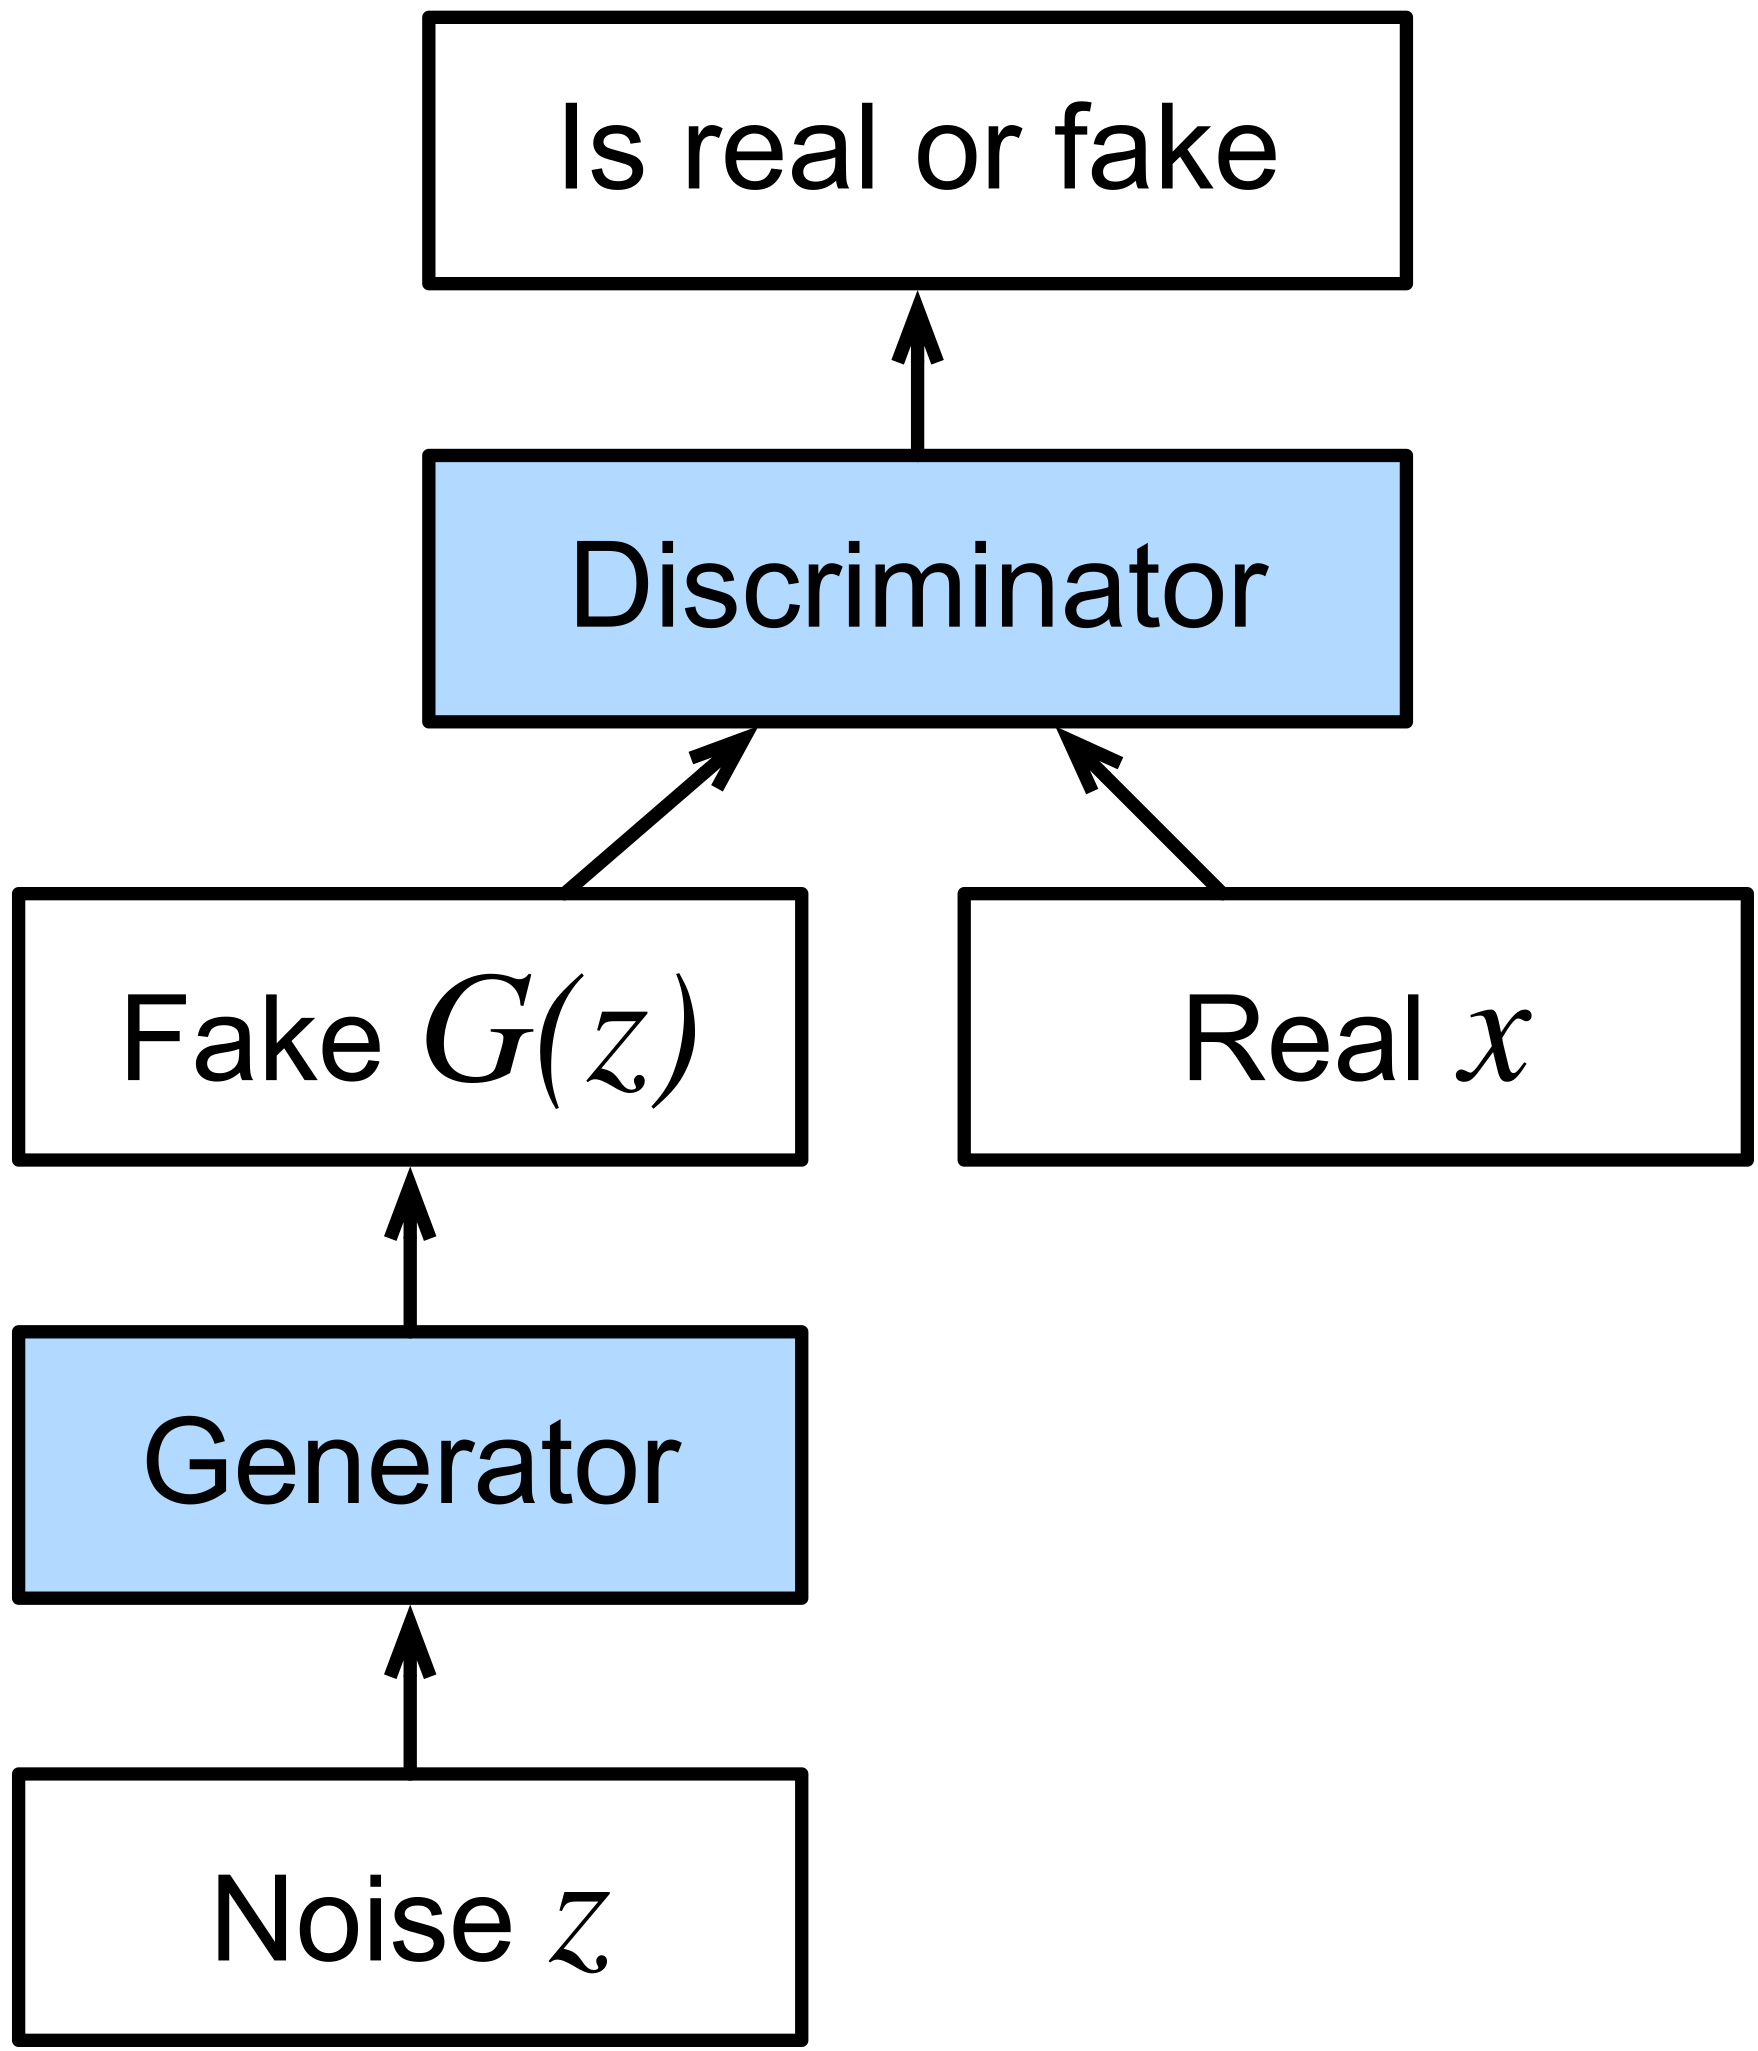
\includegraphics[height=2in]{Generative_adversarial_network.svg.png}\\
\end{center}
\end{column}
\begin{column}{.3\textwidth}
\scriptsize \url{https://commons.wikimedia.org/wiki/File:Generative_adversarial_network.svg} \normalsize
\end{column}
\end{columns}

\end{frame}

\begin{frame}{GAN -- Generative Adversarial Networks \small [cont'd]}
Image generated by a GAN:

\begin{center}
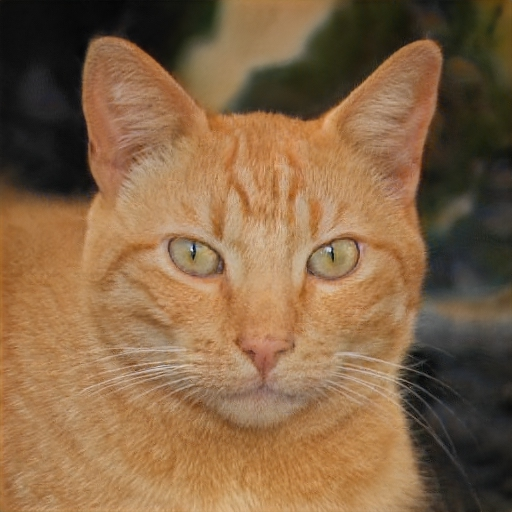
\includegraphics[height=2in]{GAN_Katze_StyleGAN2.png} \\

\scriptsize \url{https://commons.wikimedia.org/wiki/File:GAN_Katze_StyleGAN2.png} \normalsize
\end{center}

\end{frame}

%\begin{frame}[fragile]{GAN in Python}

%Load example data set:

%\begin{pythoncode}
%import keras
%import tensorflow as tf
%from keras import layers

%(x_train, y_train), (x_test, y_test) = \
                    %keras.datasets.fashion_mnist.load_data()
%x_train = x_train / 255.0
%x_test = x_test / 255.0
%\end{pythoncode}
%\end{frame}

\begin{frame}{GAN in Python}

Adapted from: 

\small\url{https://keras.io/examples/generative/dcgan_overriding_train_step/}\normalsize \\

Implementation available on the following GitHub repo:

\small\url{https://github.com/jevermann/busi4720-ai}\normalsize \\

The project can be cloned from this URL:

\small\url{https://github.com/jevermann/busi4720-ai.git}\normalsize
\end{frame}


\begin{frame}[fragile]{GAN in Python}
Discriminator receives image to classify:

\begin{pythoncode}
discriminator = keras.Sequential([
    layers.Reshape([28, 28, 1], input_shape=[28, 28]),
    layers.Conv2D(16, (3, 3), 
        padding="same", activation="relu"),
    layers.MaxPool2D((2, 2)),
    layers.Conv2D(32, (3, 3), 
        padding="same", activation="relu"),
    layers.MaxPool2D((2, 2)),
    layers.Conv2D(64, (3, 3), 
        padding="same", activation="relu"),
    layers.MaxPool2D((2, 2)),
    layers.Flatten(),
    layers.Dropout(0.2),
    layers.Dense(1, activation="sigmoid")
])
discriminator.summary()
\end{pythoncode}
\begin{itemize}
   \item In this example, the discriminator model is similar to the encoder of the AE example
\end{itemize}
\end{frame}

\begin{frame}[fragile]{GAN in Python \small [cont'd]}
Generator receives latent space vector to generate image from:

\begin{pythoncode}
latent_dim = 10

generator = keras.Sequential([
    keras.Input(shape=(latent_dim,)),
    layers.Dense(3 * 3 * 10),
    layers.Reshape((3, 3, 10)),
    layers.Conv2DTranspose(32, (3, 3), strides=2, 
        padding="valid", activation="relu"),
    layers.Conv2DTranspose(16, (3, 3), strides=2, 
        padding="same", activation="relu"),
    layers.Conv2DTranspose(1, (3, 3), strides=2, 
        padding="same", activation="sigmoid"),
    layers.Reshape([28, 28])
])
generator.summary()
\end{pythoncode}
\begin{itemize}
   \item In this example, the generator model is similar to the decoder of the AE example
\end{itemize}
\end{frame}

\begin{frame}[fragile]{GAN in Python \small [cont'd]}
Training step for a single batch of real images:
\begin{pythoncode}
class GAN(keras.Model):
    def train_step(self, real_images):
        # Sample random points in the latent space
        batch_size = tf.shape(real_images)[0]
        rnd_latent_vectors \
            = tf.random.normal((batch_size, self.latent_dim))

        # Decode them to fake images
        gen_images = self.generator(rnd_latent_vectors)

        # Combine them with real images
        images = tf.concat([gen_images, real_images], axis=0)

        # Assemble labels discriminating real from fake images
        labels = tf.concat(
            [tf.ones((batch_sz, 1)), 
            tf.zeros((batch_sz, 1))], axis=0)
        # Add random noise to the labels - important trick!
        labels += 0.05 * tf.random.uniform(tf.shape(labels))
\end{pythoncode}
\end{frame}

\begin{frame}[fragile]{GAN in Python \small [cont'd]}
Training the discriminator:
\begin{pythoncode}
        # Train the discriminator
        with tf.GradientTape() as tape:
            predictions = self.discriminator(images)
            d_loss = self.loss_fn(labels, predictions)
            
        grads = tape.gradient(
            d_loss, 
            self.discriminator.trainable_weights)
        self.d_optimizer.apply_gradients(
            zip(grads, self.discriminator.trainable_weights))
\end{pythoncode}
\end{frame}

\begin{frame}[fragile]{GAN in Python \small [cont'd]}
Training the generator:
\begin{pythoncode}
        # Sample random points in the latent space
        random_latent_vectors = \
            tf.random.normal((batch_size, self.latent_dim))

        # Assemble labels that say "all real images"
        misleading_labels = tf.zeros((batch_size, 1))

        # Train the generator 
        with tf.GradientTape() as tape:
            predictions = self.discriminator(
                self.generator(random_latent_vectors))
            g_loss = self.loss_fn(
                misleading_labels, predictions)

        grads = tape.gradient(
            g_loss, 
            self.generator.trainable_weights)
        self.g_optimizer.apply_gradients(
            zip(grads, self.generator.trainable_weights))
\end{pythoncode}
\end{frame}

%\begin{frame}[fragile]{GAN in Python \small [cont'd]}
%Training the generator:
%\begin{pythoncode}
        %# Update metrics
        %self.d_loss_metric.update_state(d_loss)
        %self.g_loss_metric.update_state(g_loss)
        %return {
            %"d_loss": self.d_loss_metric.result(),
            %"g_loss": self.g_loss_metric.result(),
        %}
%\end{pythoncode}
%\end{frame}

\begin{frame}{GAN Training}

\begin{block}{Problems}

\begin{itemize}
   \item Loss not necessarily decreaseing as generator and discriminator alternatingly improve
   \item Discriminator may ''overpower'' generator
   \begin{itemize}
       \item Reduce discriminator learning rate
       \item Remove CNN layers or reduce number of filters
       \item Add dropout layers or increase dropout
   \end{itemize}
   \item Generator may ''overpower'' discriminator
\end{itemize}
\end{block}
\end{frame}



\end{document}



